\documentclass{cpp}

\usepackage{dsfont}
\usepackage{enumerate}
\usepackage{wrapfig}
\usepackage[toc,title]{appendix}
\renewcommand{\appendixtocname}{附录}
\usepackage{setspace}

\usepackage[T1]{fontenc}
\usepackage[usefilenames,
  RMstyle={Medium,Semibold},
  SSstyle={Medium,Semibold},
  TTstyle={Medium,Semibold},
  DefaultFeatures={Ligatures=Common}]{plex-otf}
  
\lstset{
  language=C++
}

\theoremstyle{nobreak}
\theoremindent=0.0cm
\theoremheaderfont{\kern-0.0cm\normalfont\bfseries}
\newtheorem{theorem}{定理}[section]
\newtheorem{corollary}{推论}[theorem]
\newtheorem{lemma}[theorem]{引理}
\newtheorem{definition}[theorem]{定义}
\newtheorem{property}{性质}[theorem]
\newtheorem{example}{例题}[section]

\theoremstyle{nonumberplain}
\theoremindent0cm
\theoremsymbol{$\Box$}
\theoremheaderfont{\itshape}
\theoremseparator{}
\theorembodyfont{\normalfont}
\newtheorem{proof}{证明}
\newtheorem{solution}{解}

\title{\textsc{TravelAgency}: 疫情下低风险旅行模拟系统}
\subtitle{数据结构课程设计 (2020年春)}
\author[1,2]{徐逸辰}
\affil[1]{北京邮电大学,计算机学院}
\affil[2]{2018213555}
\email{linyxus@bupt.edu.cn}

\begin{document}

\maketitle

%\begin{abstract}
%TODO
%\end{abstract}

\setcounter{tocdepth}{1}
\tableofcontents

\newpage

\section{引言}

在本文中,我将介绍\textsc{TravelAgency}:新冠疫情环境下的低风险旅行规划模拟系统。该系统能够根据各个城市的风险等级,以及城市之间的线路信息,基于两种不同的策略,为用户模拟规划出低风险的旅行方式。

系统实现了所有必须完成的需求,包含基于两种策略的规划:最小风险旅程与带时间约束的最小风险旅程(也即限时最小风险)。并且实现了所有选作请求,能够在地图上实时绘制出旅程的状态,并且考虑到了旅行线路带来的风险。系统使用了高效的数据结构,利用图来描述城市线路信息,利用邻接表来存储图,利用可持久化链表来描述旅程;使用SPFA作为两种策略的规划算法,通过对系统的性能测试展现了系统的效率。

系统由多种语言完成开发,大抵可分为三个部分。(a) 图形用户界面,由前端技术实现,由 HTML、CSS和JavaScript进行开发。采用Vus.js作为前端框架,并且调用了高德地图API,实现绘制城市信息,实时显示旅行线路与状态;(b) 算法核心,由C++进行开发,采用了图作为城市线路的数据结构,利用可持久化链表作为描述旅程的数据结构,实现了较高的空间效率。且应用SPFA实现了高效的线路规划;(c) 服务器。前端技术实现的用户界面需要和C++实现的高效算法逻辑进行通信,为了实现他们之间高效、简单的通信,使用Python开发了WebSocket服务器。一方面,服务器使用WebSocket与前端用户界面通信,另一方面,利用 \lstinline{ctypes} 库调用C++算法核心的动态库。起到了桥接作用。

\begin{figure}[h]
\centering
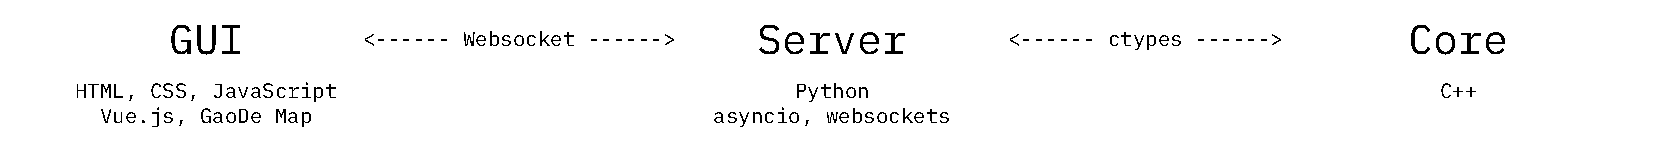
\includegraphics[width=\textwidth]{figures/language_arch}
\caption{系统架构}
\label{fig:language-arch}
\end{figure}

本文将分几个部分介绍\textsc{TravelAgency}旅行规划模拟系统的各方面。在第 \ref{sec:preliminary} 节中,将介绍\textsc{TravelAgency}的背景,需求功能分析与设计概要。在第 \ref{sec:showcase} 节中,将展示系统功能,解说系统的基本特性。在第 \ref{sec:design} 节中,将细致地讲解系统的设计,包含数据结构、算法,以及前端、服务器的设计概述。在第 \ref{sec:experiments} 节中,将讲述样例的基本信息以及运行结果分析。在第 \ref{sec:conclusion} 节中,将进行总结讨论,指出系统的优点与改进之处。除此以外,在附录 \ref{sec:compile-and-run} 中详细介绍了运行、编译工程的方法。在附录 \ref{sec:manual} 中给出了系统的用户使用说明。在附录 \ref{sec:perf-test} 展示了系统性能测试的结果。

\section{背景}
\label{sec:preliminary}

\paragraph{系统背景}

\textsc{TravelAgency}的背景是在新冠疫情环境下,对低风险旅行的规划与模拟。新冠疫情以来,全国上下团结一心,共同抵抗疫情,然而也未出行带来的诸多不便。如今疫情已经受到控制,然而出行仍然具有一定风险。\textsc{TravelAgency}旨在根据城市风险等级、线路信息等条件,为用户规划出合理的、有或没有时间限制的最低风险路线。

\paragraph{城市风险等级与等待风险}

系统假设城市风险分为三级:高风险、中风险、低风险。且具有各自的风险系数,如表 \ref{tab:city-level-risk} 所示。
\begin{table}[h]
\centering
\begin{tabular}{cccc}
\toprule
风险等级 & 低 & 中 & 高 \\
\midrule
风险系数 & 0.2 & 0.3 & 0.9 \\
\bottomrule
\end{tabular}
\caption{城市风险系数表}
\label{tab:city-level-risk}
\end{table}

假设某一旅客在$t_a$到达城市$c$,城市$c$具有风险系数$r_c$,且他下面要进行的旅行线路在$t_d$出发。则因等待而产生的风险定义为
\begin{equation}
  R_w \triangleq \| t_d - t_a \| \cdot r_c,
\end{equation}
其中,$\| t_d - t_a \| \triangleq (t_d - t_a + 24) \% 24$为需要等待的时间。

\paragraph{线路信息与路程风险}

系统假设一条线路由如下信息定义:出发地点、目的地点、出发时间、所用时长、类型。系统假设所有系统都以一天为周期重复,因而任一线路的出发时间$t_d$满足$t_d = 0, 1, 2, \cdots, 23$。线路时长没有限制。线路类型有三种:飞机、火车、客车。不同类型的线路具有不同的风险系数,如表 \ref{tab:line-type-risk} 所示。
\begin{table}[h]
\centering
\begin{tabular}{cccc}
\toprule
线路类型 & 客车 & 火车 & 飞机 \\
\midrule
风险系数 & 2 & 3 & 9 \\
\bottomrule
\end{tabular}
\caption{线路风险系数表}
\label{tab:line-type-risk}
\end{table}

而假设某一线路$l$从城市$c$出发,时长为$\tau$。$l$和$c$分别具有风险系数$r_l$与$r_c$。则此条线路带来的路程风险定义为
\begin{equation}
  R_t \triangleq r_l \tau r_c.
\end{equation}

\paragraph{城市地图}

将城市信息与线路信息建模为一张图,定义$\mathcal G = (\mathcal V, \mathcal E, r_c, r_l, t_d, t_a, \tau, v_s, v_d)$。其中$\mathcal V = \{ c_1, c_2, \cdots, c_n \}$为城市集合,$\mathcal E = \{ l_1, l_2, \cdots, l_k \}$为线路集合。$r_c : \mathcal V \rightarrow \mathds R$为城市到其风险系数的映射。$r_l : \mathcal E \rightarrow \mathds R$为线路到其风险系数的映射。$t_d, t_a : \mathcal E \rightarrow \{ 0, 1, \cdots, 23 \}$为线路到其出发、到达时间的映射。$\tau : \mathcal E \rightarrow \mathds N_+$为线路到其时长的映射。而$v_s, v_d : \mathcal E \rightarrow \mathcal V$为线路到其出发、目的城市的映射。可以知道,一般来说这张图是有向多重图。

\paragraph{旅行规划与两种策略}

系统需要解决的是低风险旅行规划问题。假设某一旅客在$t_0$时从城市$c_0$出发,希望到达城市$c$。系统需要模拟规划出旅程,经过线路$l_0, l_1, l_2, \cdots, l_k$。可以知道这些线路满足:$v_d(l_i) = v_s(l_{i+1}), i = 0, 1, \cdots, k-1$,且$v_s(l_0) = c_0$,$v_d(l_k) = c$。而总风险可以写为
\begin{equation}
  R(l_0, l_1, \cdots, l_k) = \sum_{i=0}^k \left[ \tau_i r_c(c_i) + r_l(l_i) \tau(l_i) r_c(c_i) \right],
\end{equation}
其中,$\tau_i$为等待时间,有$\tau_0 = \| t_d(l_0) - t_0 \|, \tau_i = \| t_d(l_i) - t_a(l_{i-1}) \|, i = 1, 2, \cdots, k-1$。而$c_i = v_s(l_i), i = 0, 1, \cdots, k$为出发城市。系统需要找到符合条件的线路列表,使得$R$最小,也即如下的最优化问题
\begin{equation}
  \begin{aligned}
    \min_{l_0, \cdots, l_k} \quad & R(l_0, l_1, \cdots, l_k) \\
    \text{s. t.} \quad & v_d(l_i) = v_s(l_{i+1}), i = 0, 1, \cdots, k-1 \\
    & v_s(l_0) = c_0, v_d(l_k) = c \\
  \end{aligned}
\end{equation}
而对于带有时间约束的最小风险策略,旅途总时长可以类似地写为
\begin{equation}
  T(l_0, l_1, \cdots, l_k) = \sum_{i=0}^k \left[ \tau_i + \tau(l_i) \right].
\end{equation}
假设有时间约束$T \le \Gamma$,则限时最小风险策略可以被认为是求解下列最优化问题
\begin{equation}
  \begin{aligned}
    \min_{l_0, \cdots, l_k} \quad & R(l_0, l_1, \cdots, l_k) \\
    \text{s. t.} \quad & v_d(l_i) = v_s(l_{i+1}), i = 0, 1, \cdots, k-1 \\
    & v_s(l_0) = c_0, v_d(l_k) = c \\
    & T(l_0, l_1, \cdots, l_k) \le \Gamma \\
  \end{aligned}
\end{equation}




\section{系统功能与展示}
\label{sec:showcase}

\begin{figure}[t]
	\centering
	\subfloat[概览]{
		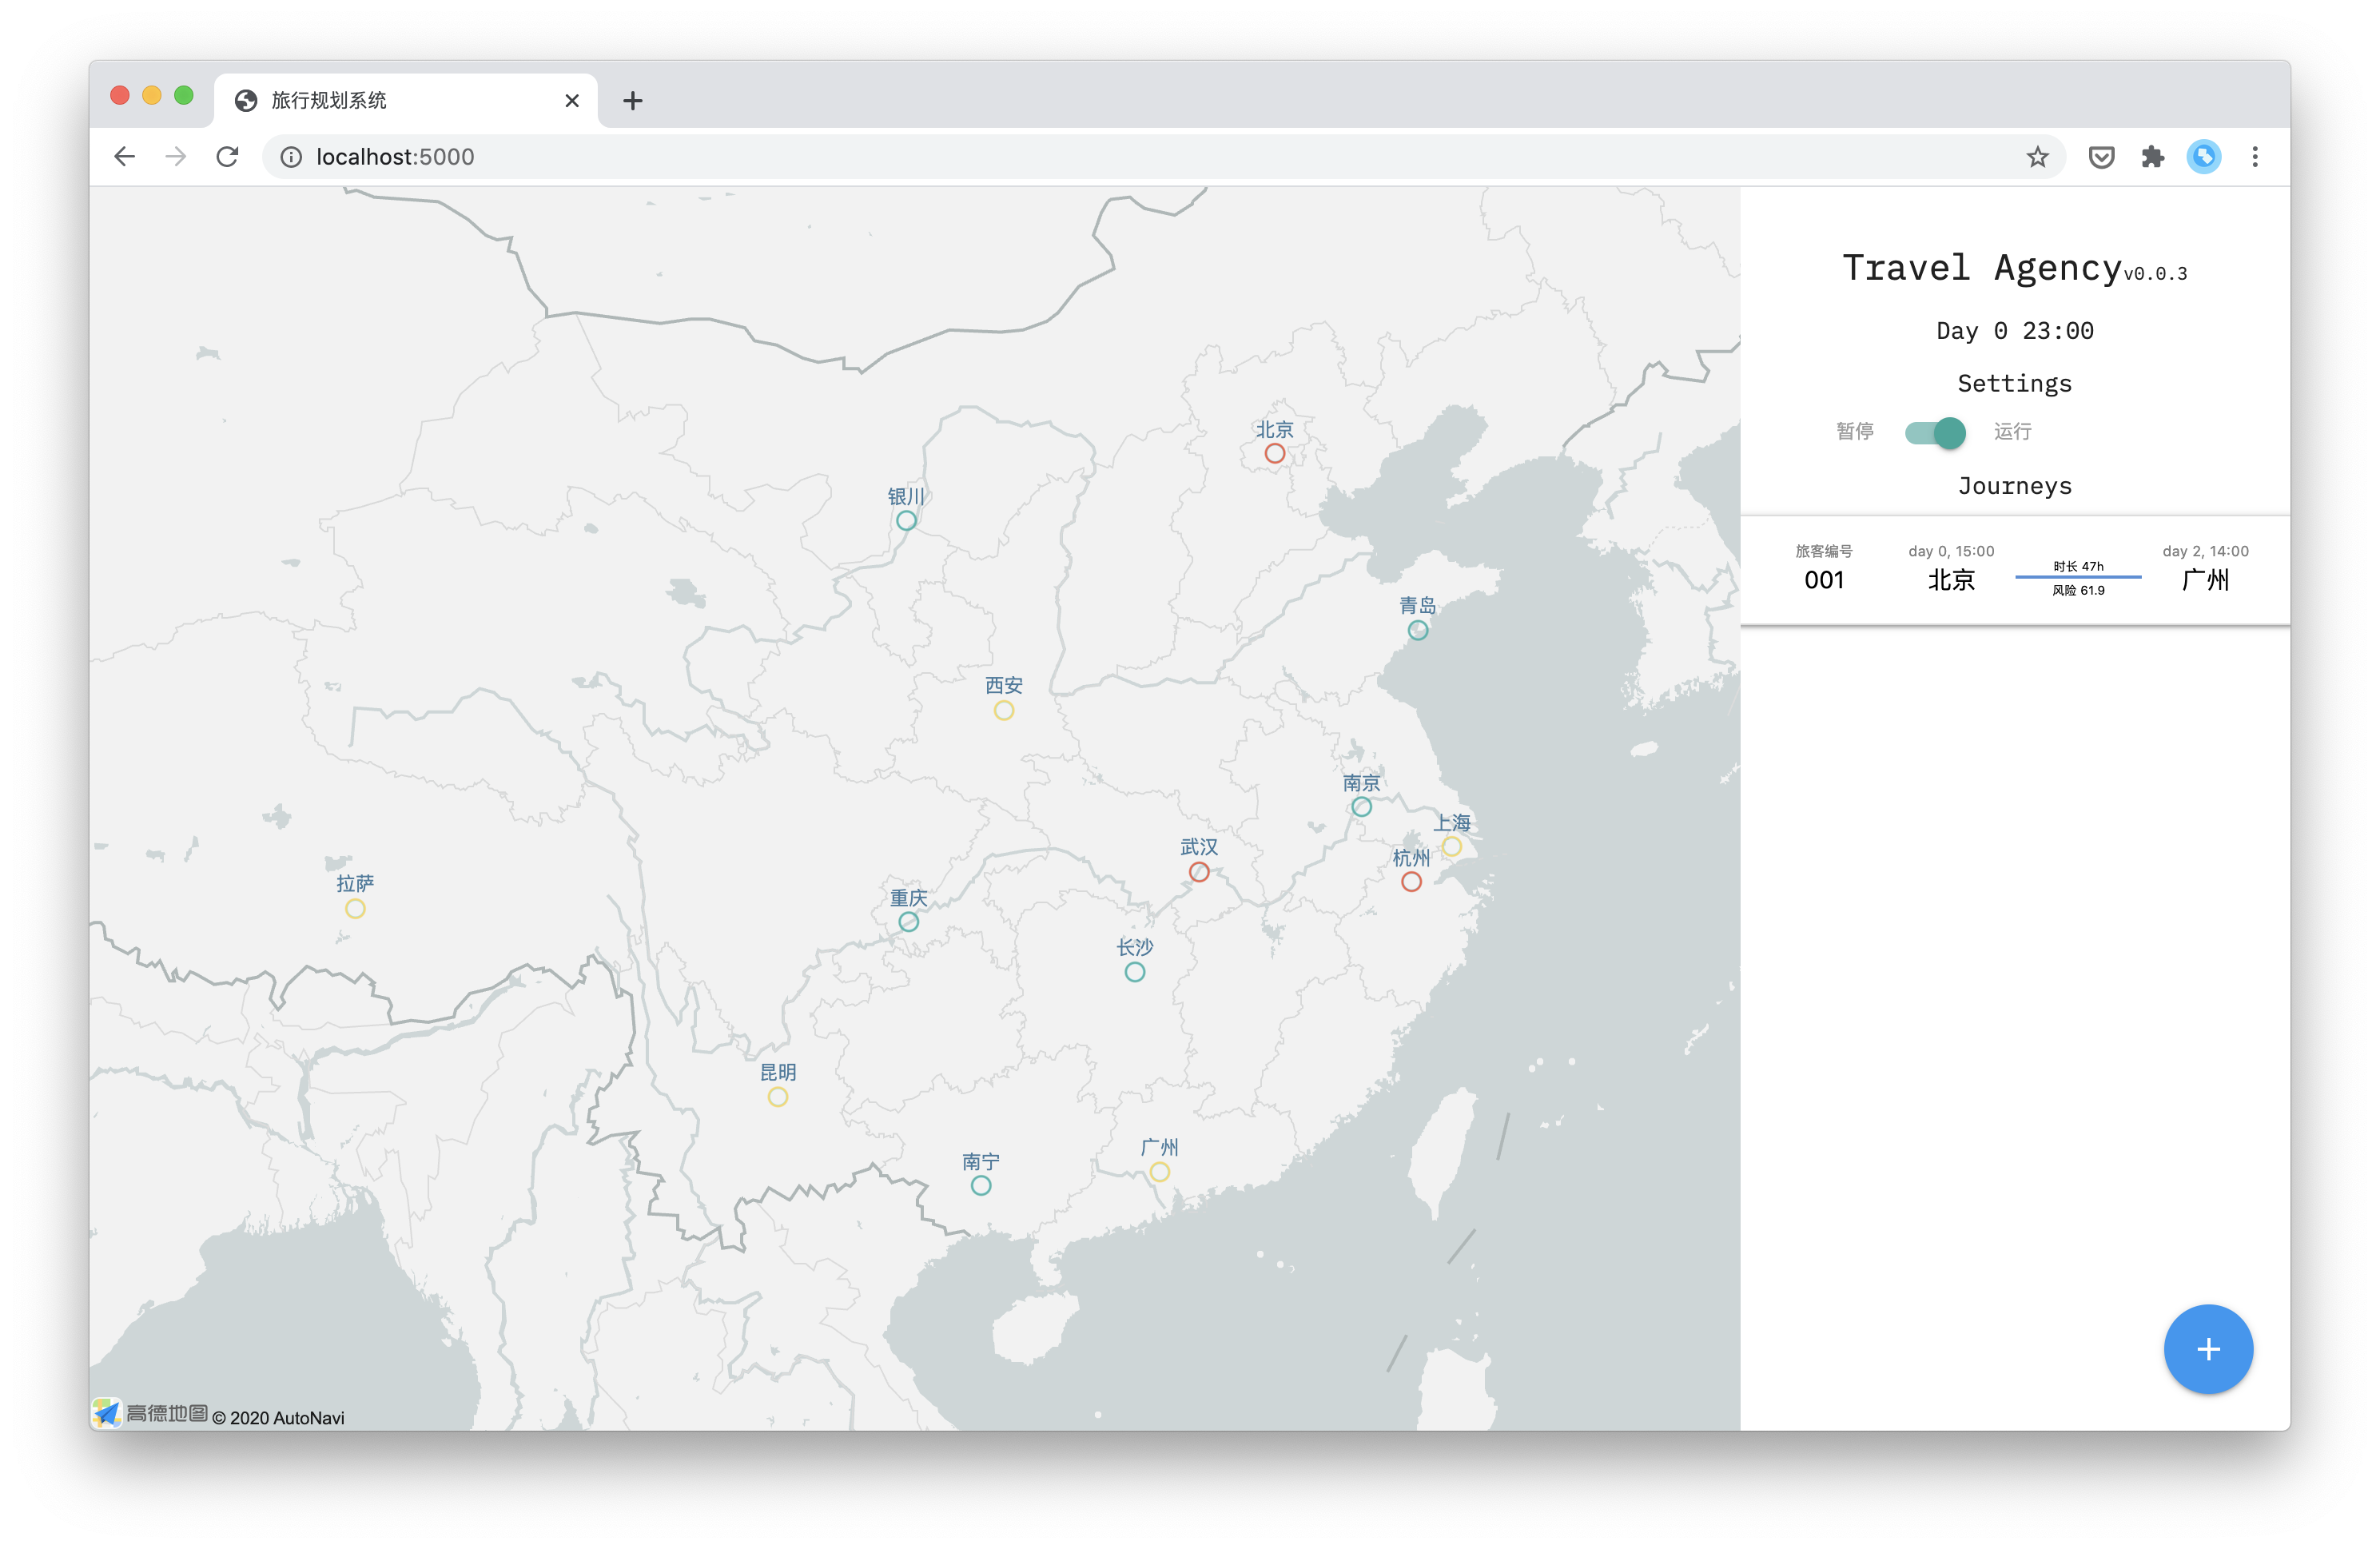
\includegraphics[width=0.5\textwidth]{figures/screenshot_overview}
		\label{fig:showcase-overview}
	}
	\subfloat[旅程状态]{
		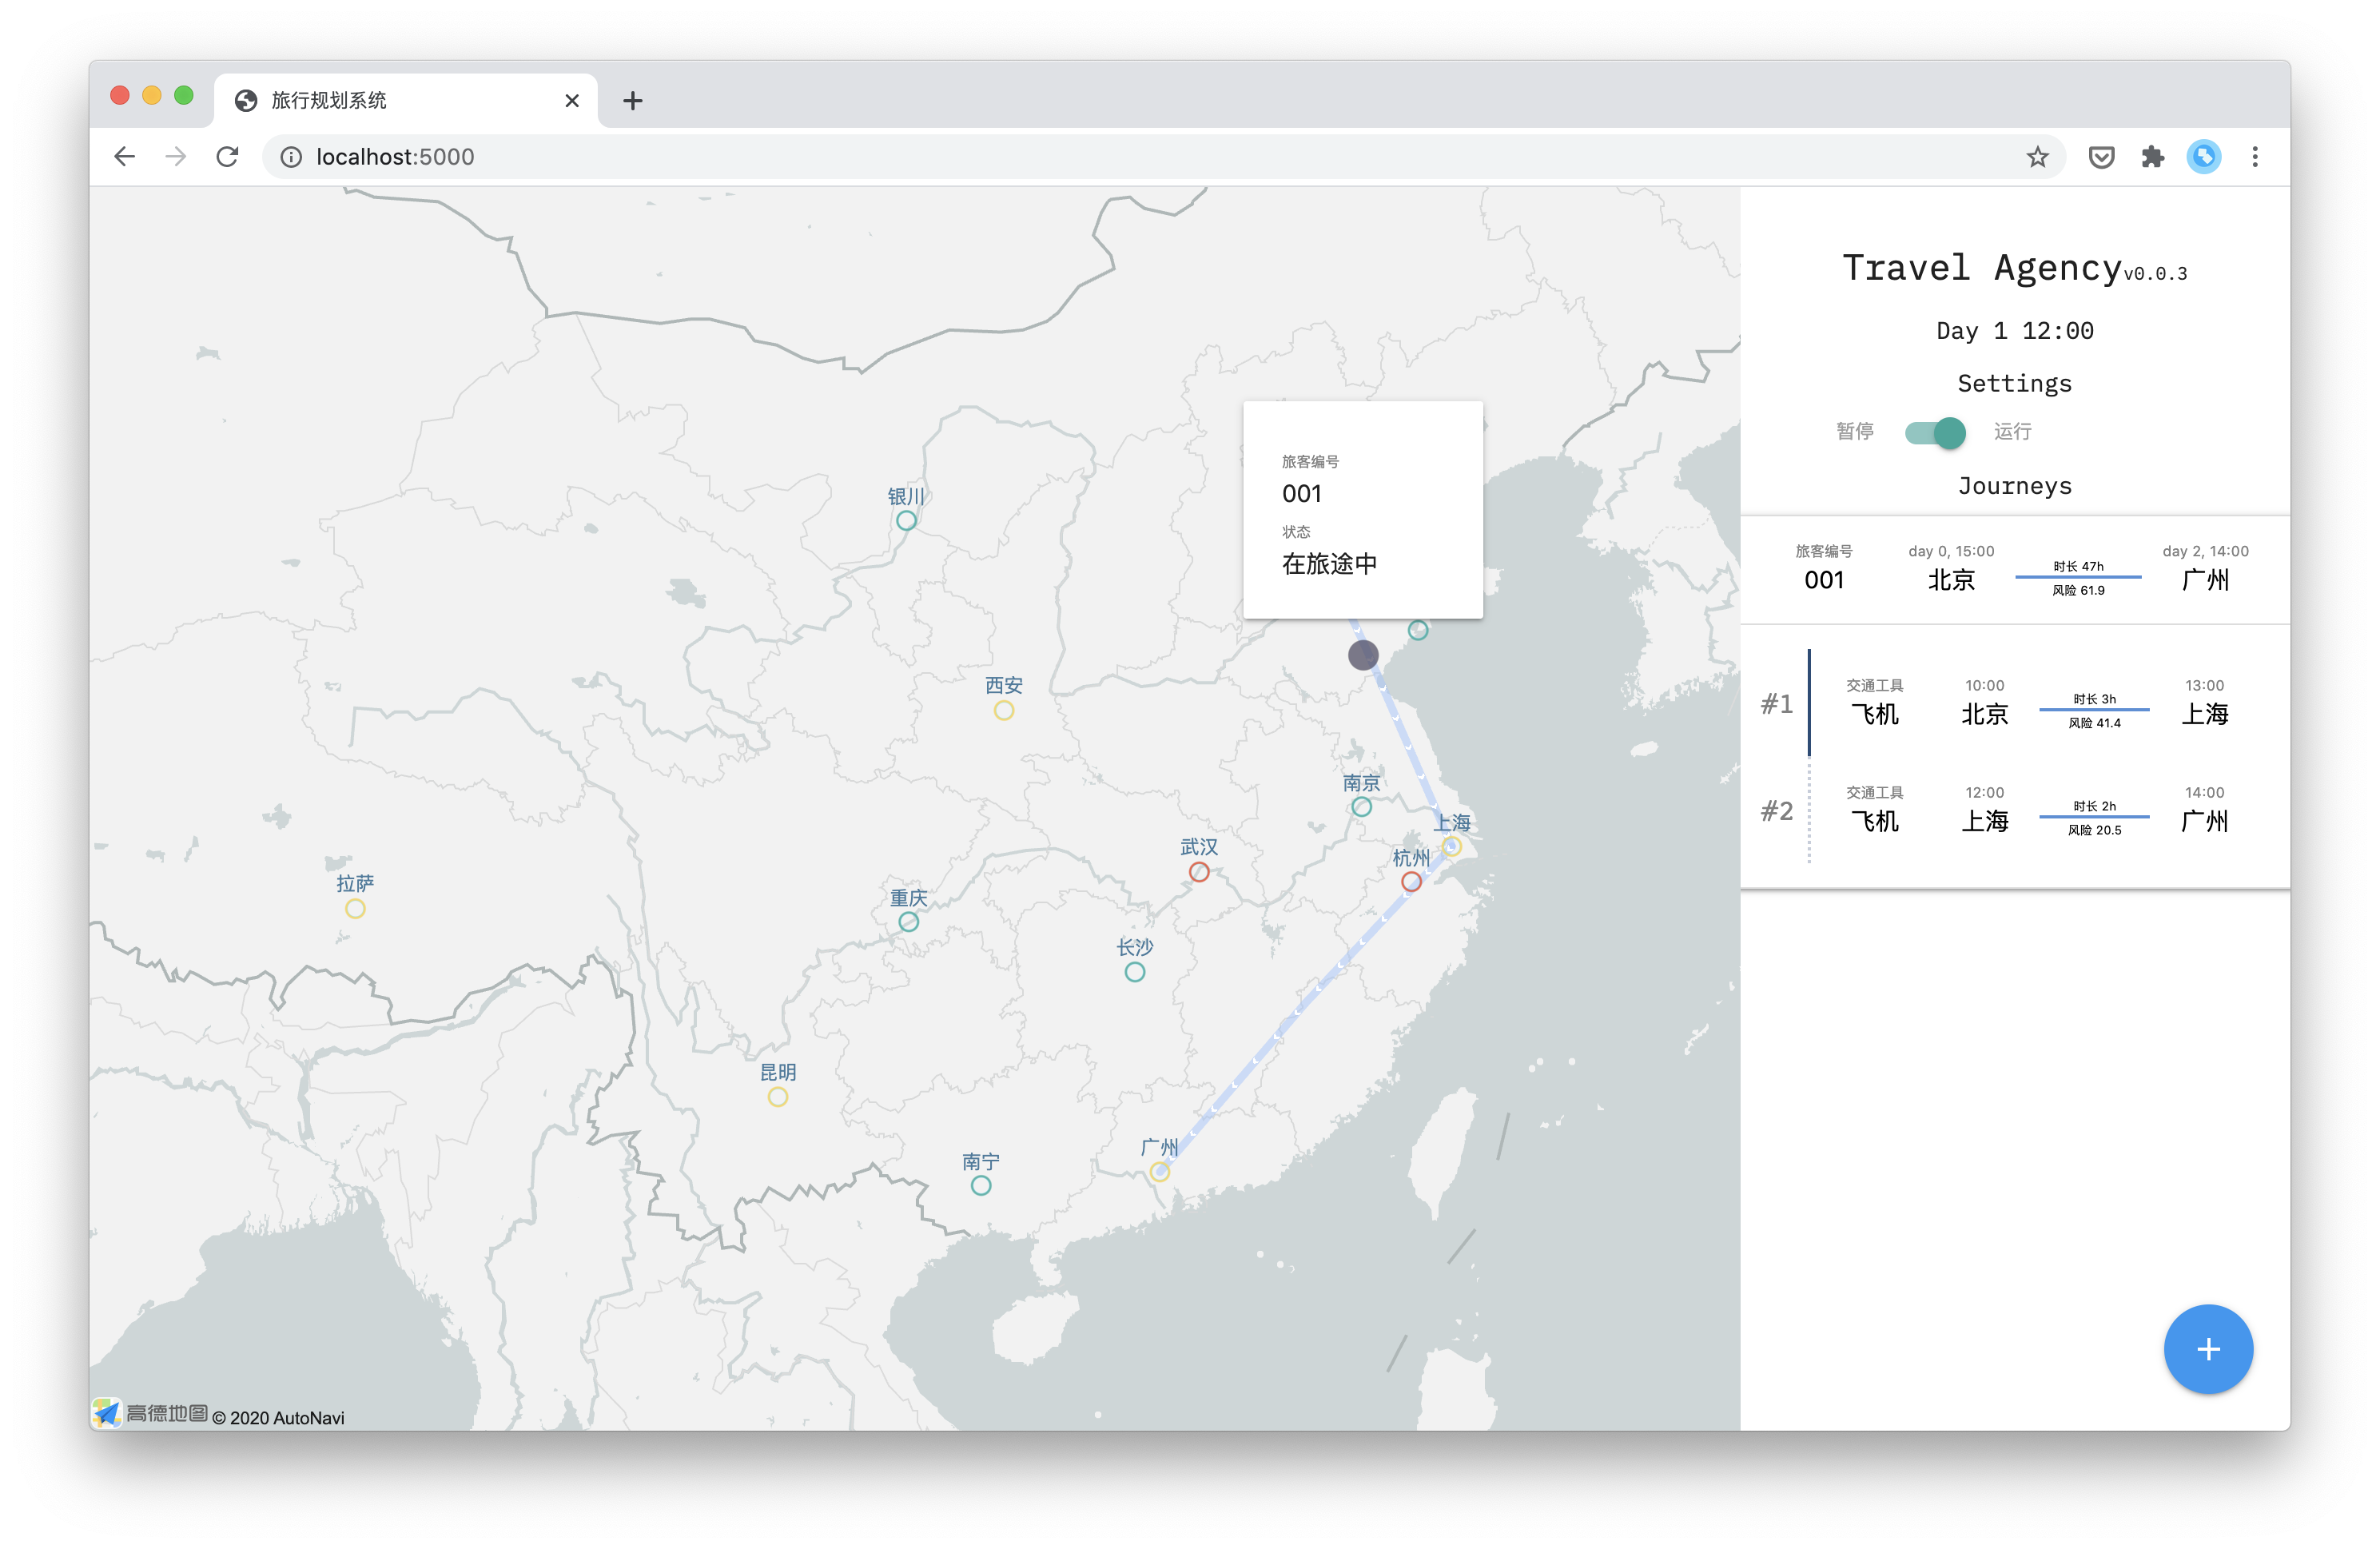
\includegraphics[width=0.5\linewidth]{figures/screenshot_journey_details}
		\label{fig:showcase-journey-details}
	}
	\caption{系统界面概览}
	\label{fig:showcase}
\end{figure}

本小节将简单地展示\textsc{TravelAgency}系统,并且概述系统功能。

\subsection{系统界面}

图 \ref{fig:showcase} 展示了\textsc{TravelAgency}系统的界面。可以看到系统界面分为两个部分。

\begin{enumerate}[(a)]
  \item 地图。显示城市信息,也能实时显示旅途信息。对于旅途信息,会绘制旅途中搭乘的线路,以及旅客当前所在位置。将鼠标移到旅客图标上,会给出旅客号、当前状态等更加具体的信息。如图 \ref{fig:showcase-journey-details} 中所示。
  \item 信息面板。信息面板中包含了各类信息,包括:当前时间,当前进行中的旅程。点击旅程列表中的某一旅程,将显示出旅程的详细信息,包括每一步搭乘的线路、每一步所花费的时间、带来的旅程风险等等。同时,信息面板中也包含控制系统暂停运行的按钮,以及添加旅程的按钮(右下角加号按钮)。
\end{enumerate}

\begin{figure}[t]
	\centering
	\subfloat[添加旅程]{
		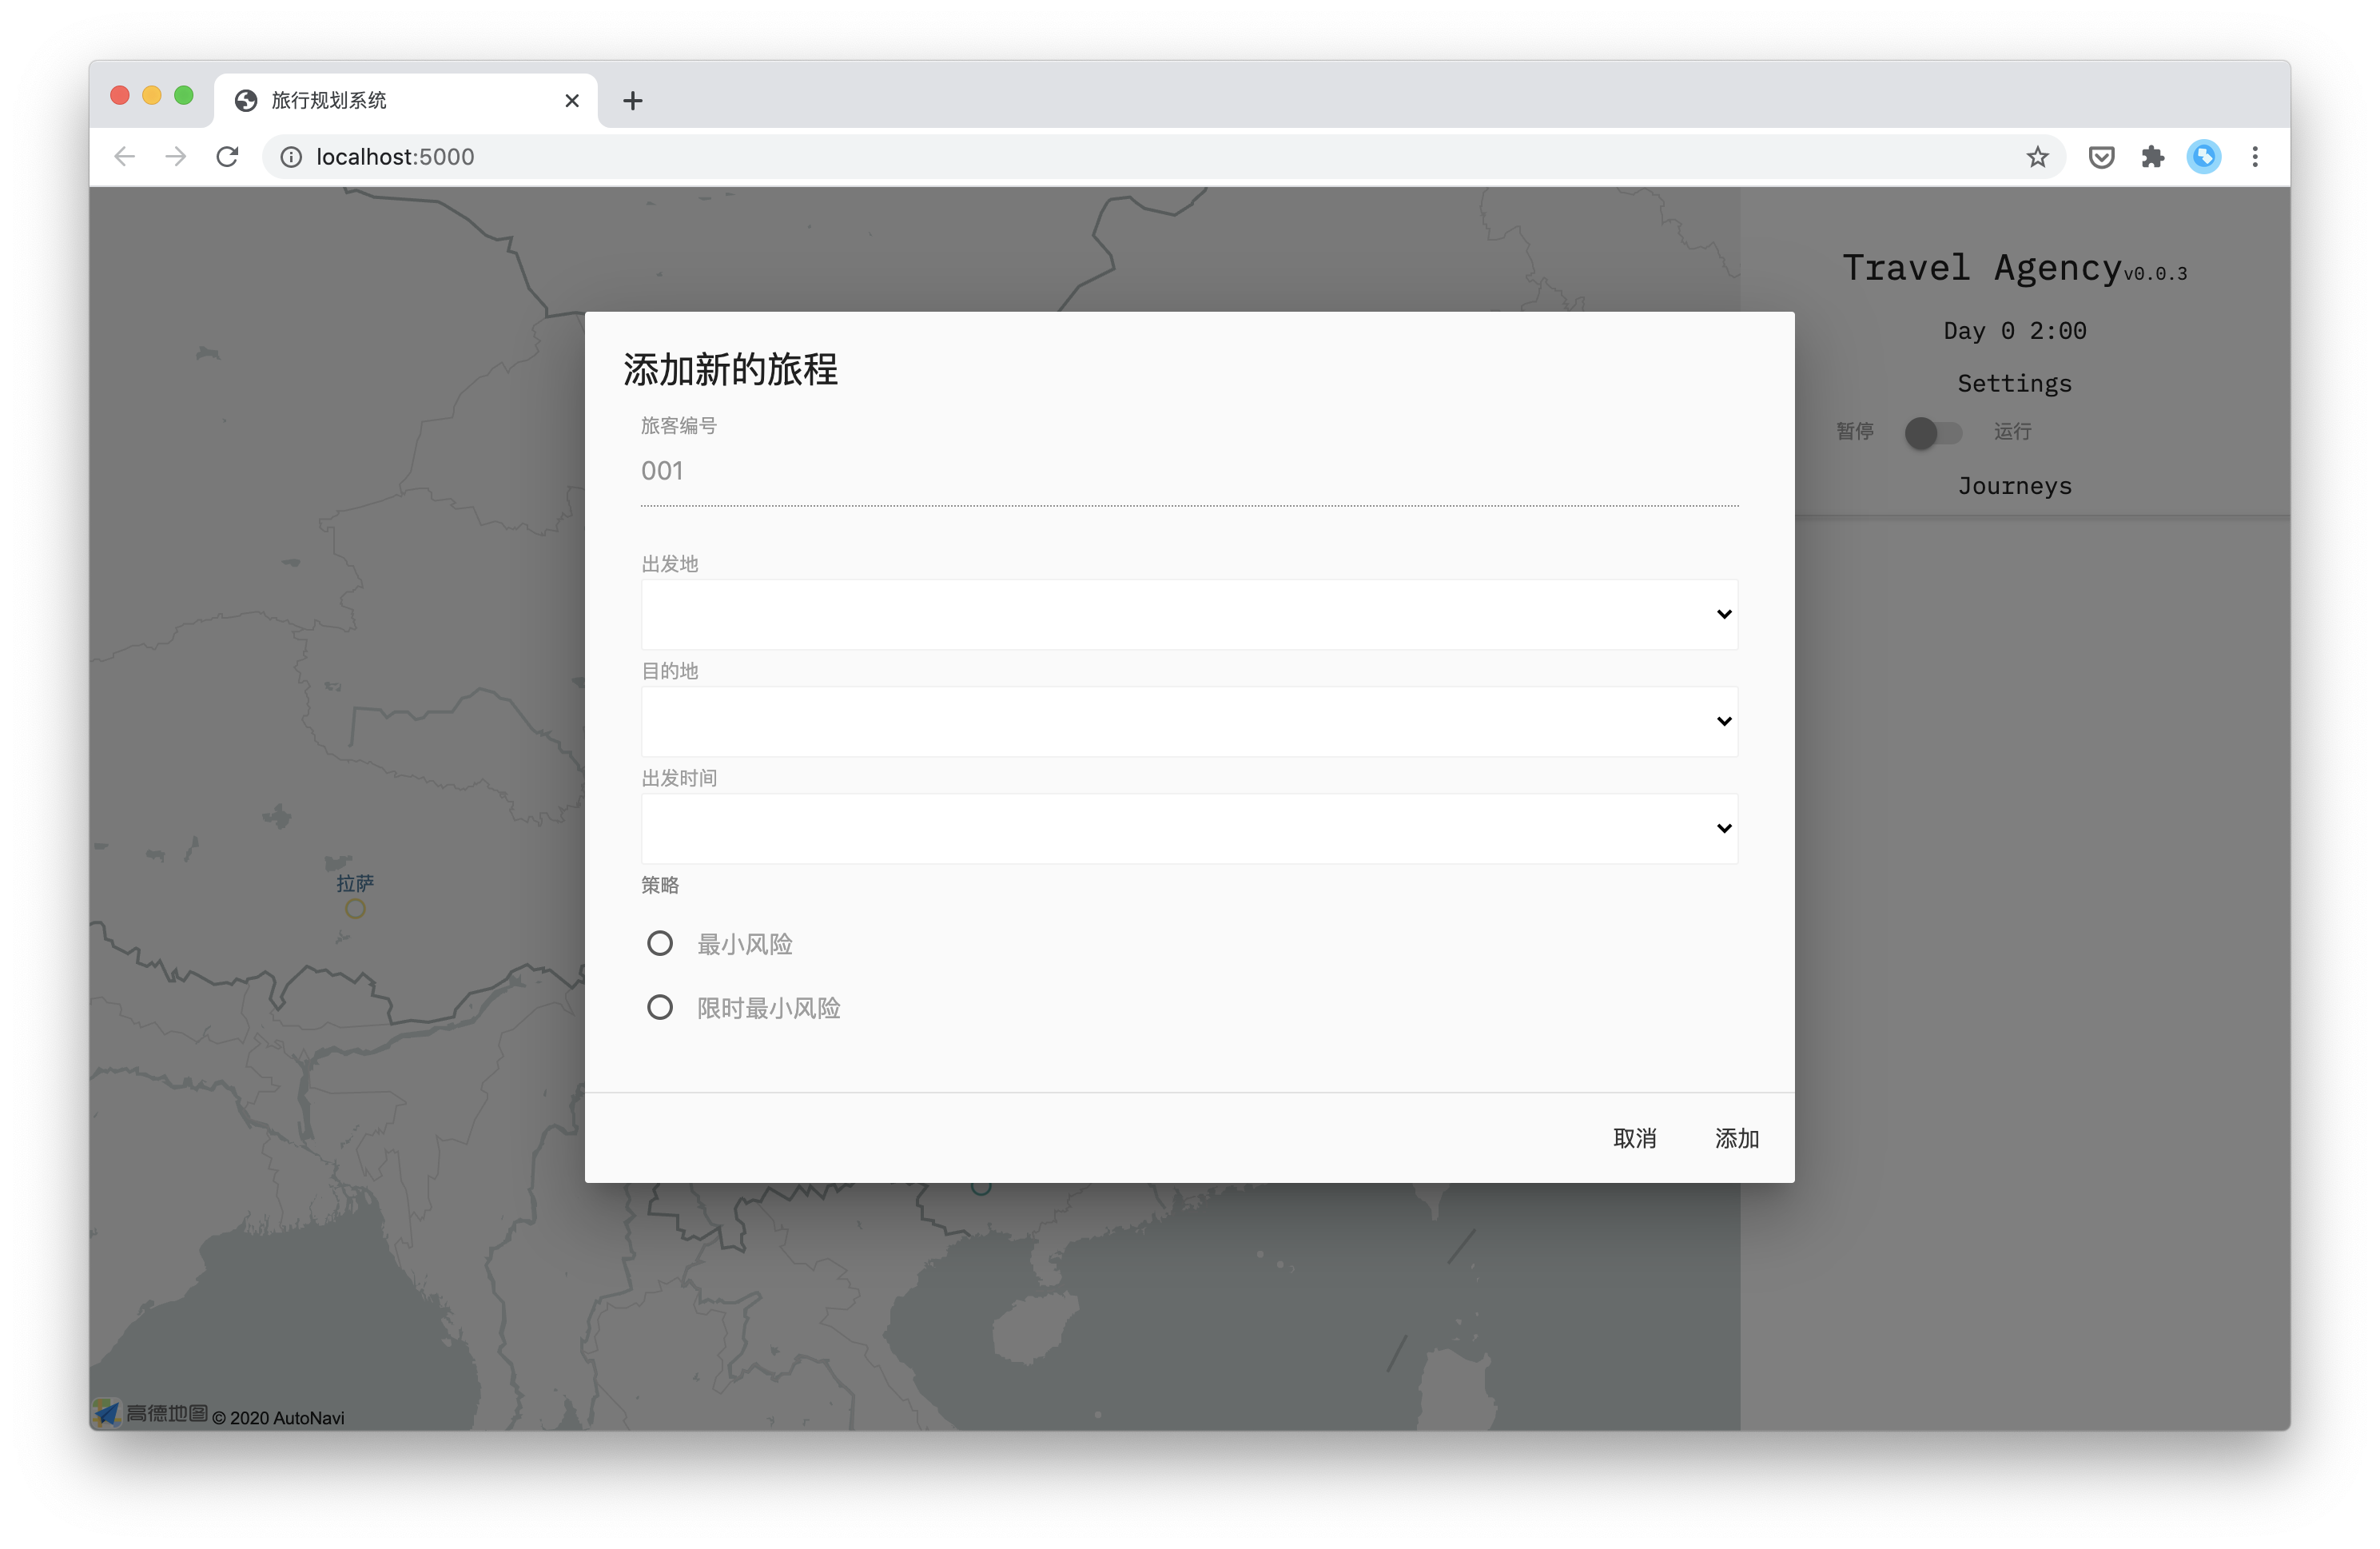
\includegraphics[width=0.5\textwidth]{figures/screenshot_add_journey}
		\label{fig:showcase-add-journey}
	}
	\subfloat[预览旅程信息]{
		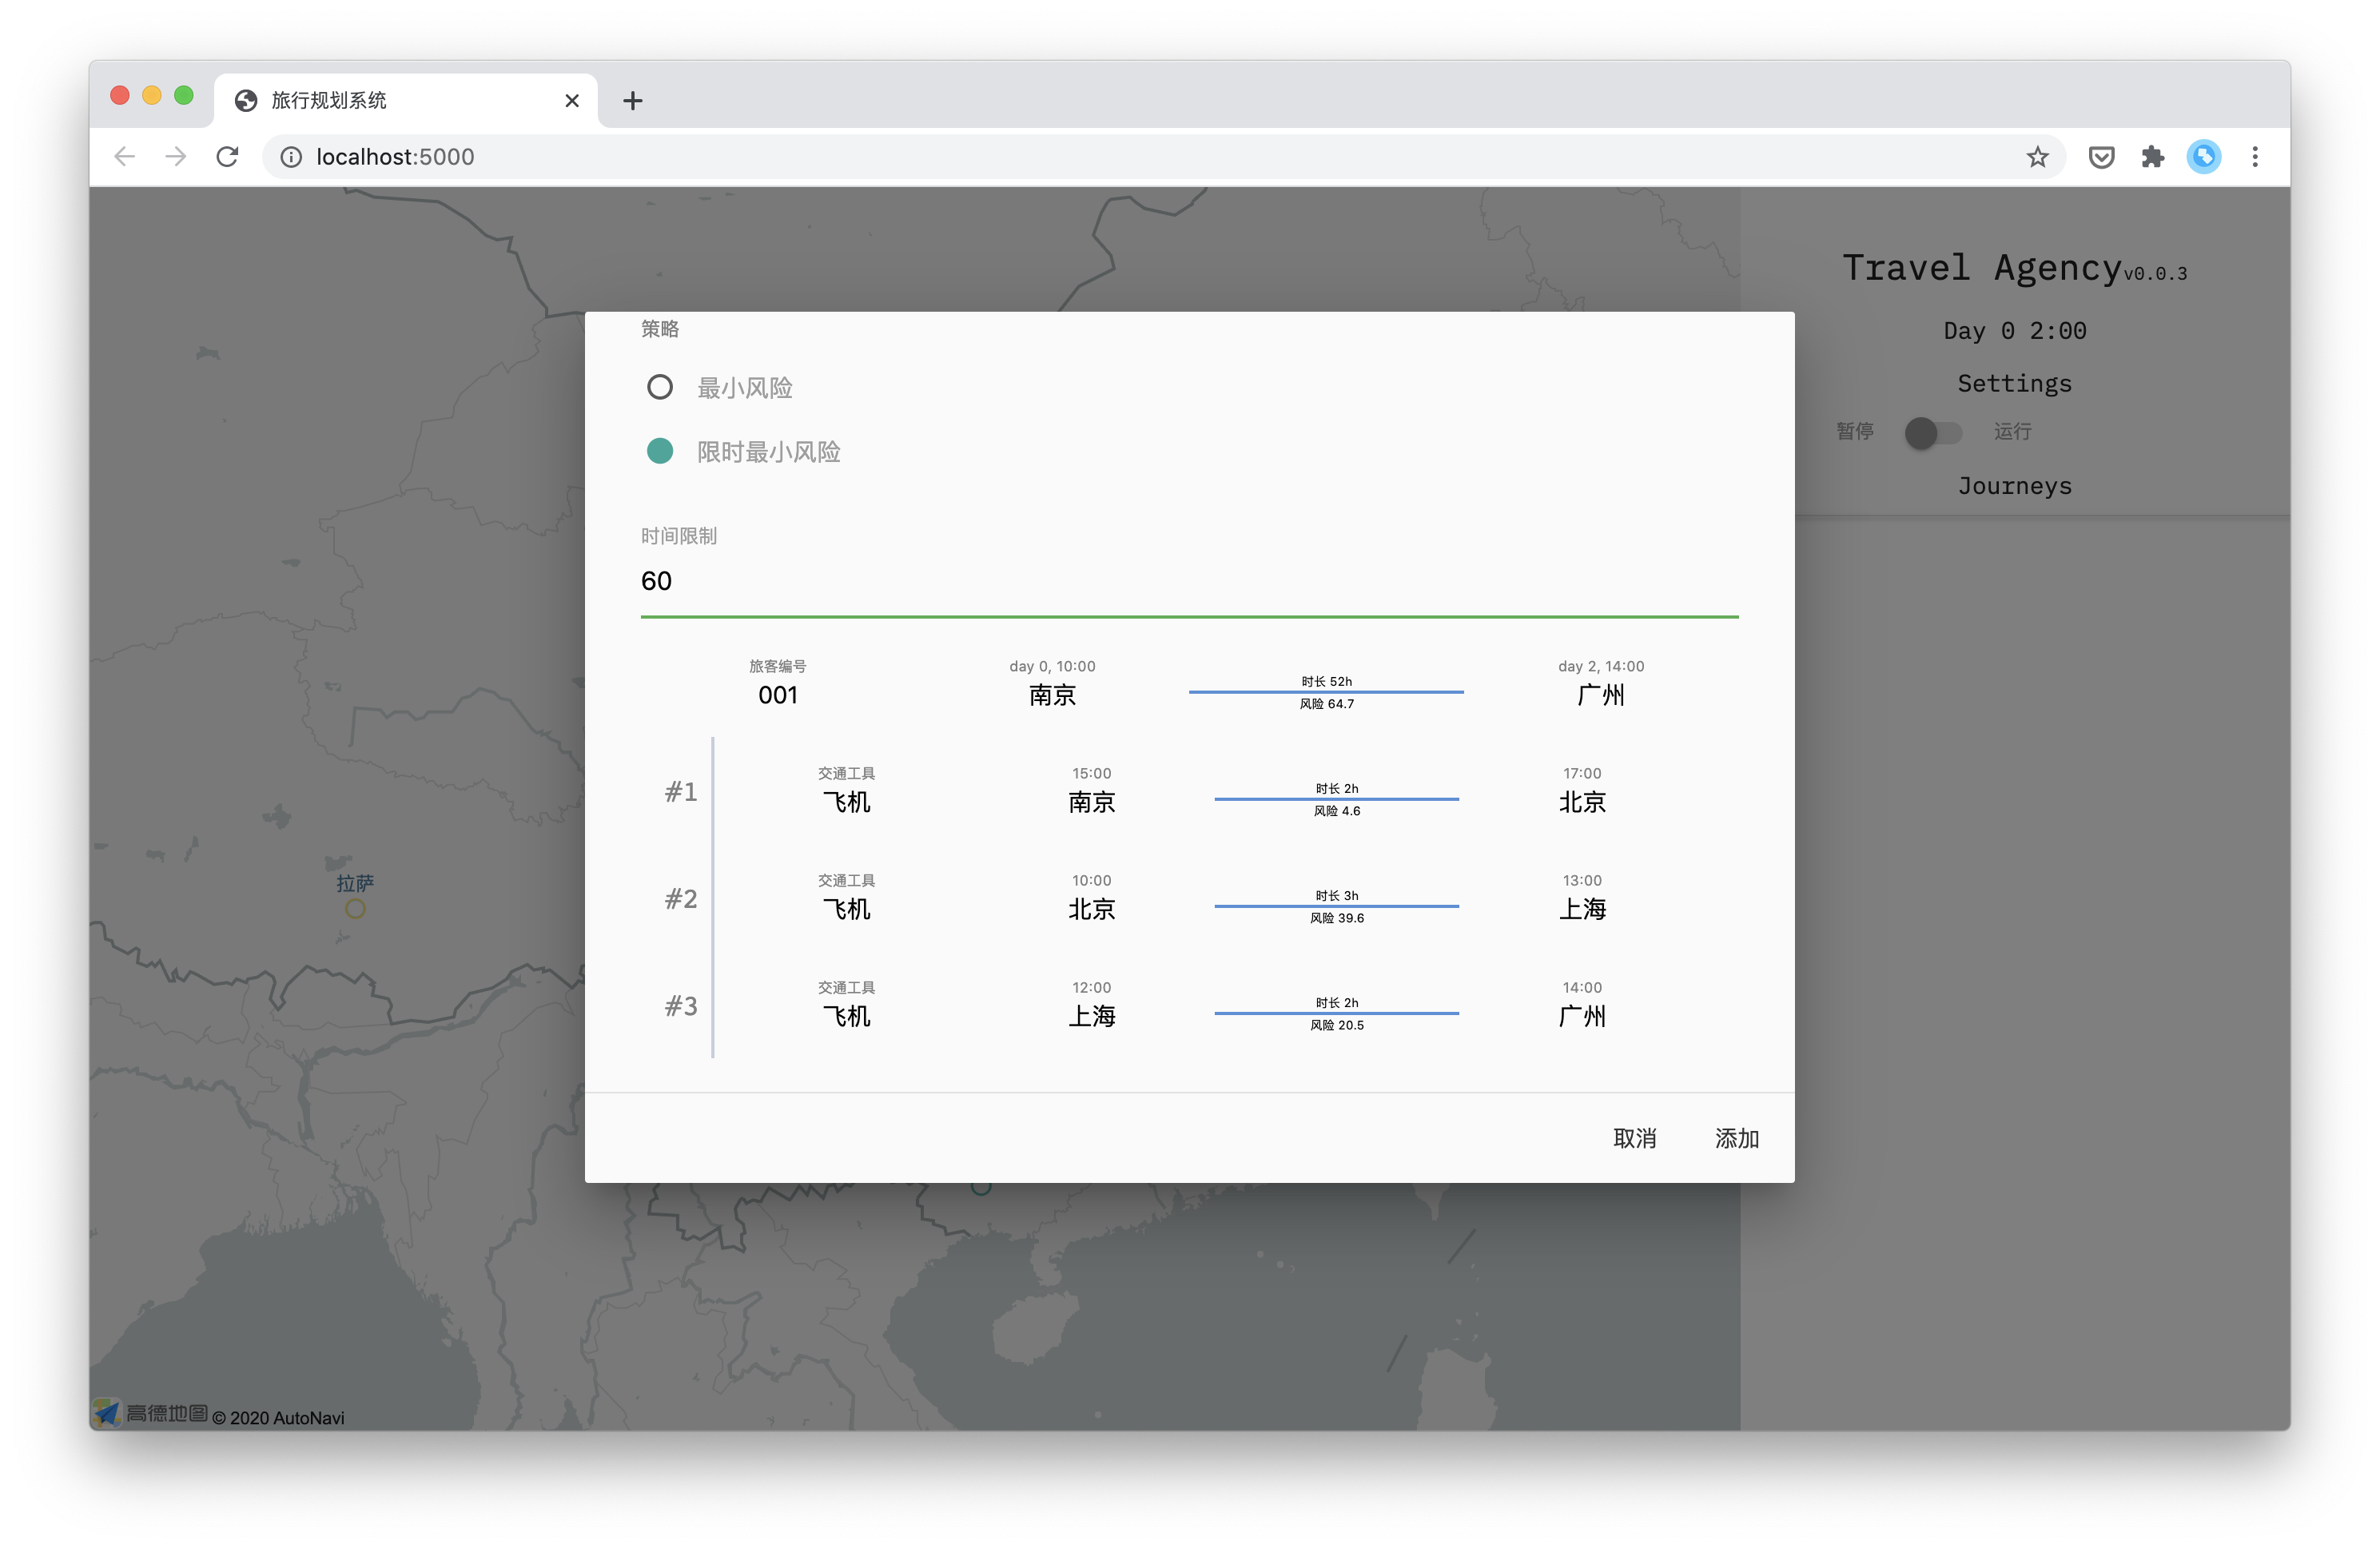
\includegraphics[width=0.5\linewidth]{figures/screenshot_add_journey_preview}
		\label{fig:showcase-add-journey-preview}
	}
	\caption{添加旅程界面}
	\label{fig:showcase-2}
\end{figure}

而图 \ref{fig:showcase-2} 中展示了在点击添加旅程的按钮之后,弹出的添加旅程界面。在这一见面中,需要输入新旅程的各类信息:出发地点、目的地点、出发时间、旅行策略,若旅行策略为限时最小风险策略,还需要输入时间限制。如图 \ref{fig:showcase-add-journey-preview} 中所示。

在输入完旅程信息之后,系统能够自动加载规划出的旅行方案,如图 \ref{fig:showcase-add-journey-preview} 中所示。旅行方案包含总时间、总风险,以及每一步的详细信息等。在确认无误之后,点击添加,就能将旅程添加到系统中。若对信息进行修改,在修改完成后,系统会自动更新显示修改后的旅行方案。点击取消,就能取消添加新的旅行。

注意到,在添加旅行的过程中,系统时间自动处于暂停状态。在取消添加或者确认添加之后,系统时间会自动恢复运行。

\subsection{系统主要功能}

系统包含以下主要功能:

\definecolor{high-risk}{HTML}{ED553B}
\definecolor{mid-risk}{HTML}{F6D55C}
\definecolor{low-risk}{HTML}{3CAEA3}

\begin{enumerate}[(a)]
  \item \textbf{显示城市地图}。如图 \ref{fig:showcase-overview} 中所示,系统能够将城市显示在地图上。用不同颜色的圈来表示不同的风险等级。具体地,\textit{{\color{high-risk}红色}}代表高风险地区;\textit{{\color{mid-risk}黄色}}代表中风险地区;\textit{{\color{low-risk}绿色}}代表低风险地区。
  \item \textbf{两种策略的低风险旅行规划}。\textsc{TravelAgency}能够实现最小风险、限时最小风险策略的旅行规划。\textit{且不仅能考虑到等待带来的风险,也能够考虑到旅程中的风险}。
  \item \textbf{实时显示旅行状态}。系统能够实时显示旅行的状态。能够将旅行线路绘制在地图上,并且显示旅客所处位置与状态,如:等待出发,在旅途中,正在等候,已抵达。且能直观、美观地显示出每条旅程的详细信息。
  \item \textbf{暂停、继续系统时间}。系统能够自由地暂停、继续时间运行。当添加旅行时,系统时间自动停止。
\end{enumerate}










\section{系统设计}
\label{sec:design}

本小节将介绍系统设计。首先,简单地回顾系统整体架构。随后介绍算法核心中的模块设计与调用关系。接着,介绍算法核心中的数据结构与规划算法。最后,简要介绍服务器端与前端的模块结构关系与大概设计。

\begin{figure}[t]
  \centering
  
\includegraphics[width=\textwidth]{figures/system_arch}
  \caption{系统架构}
  \label{fig:system-arch}
\end{figure}

\subsection{系统架构}

如图 \ref{fig:system-arch} 中所示,系统由三大部分组成。(a) GUI负责信息展示、旅程展示、用户交互等。与服务器通信;(b) 服务器负责与GUI通信。管理已有的旅程信息。并且调用算法核心进行旅程规划;(c) 算法核心能够加载、管理城市线路信息,进行旅行规划,生成旅途信息等等。

\textsc{TravelAgency}系统的核心逻辑功能,都在算法核心中实现,包括:定义了城市线路信息的数据结构(图),从文件中加载读取城市、线路信息;定义了描述旅程的数据机构(可持久化链表),规划并生成旅程信息。注意当前旅程信息的保管不由算法核心完成,而由服务器完成,服务器将所有规划模拟的旅行保存在一个列表中,能够通过Websocket提供给前端用户界面。

程序当前的状态,包括当前时间,进行中的旅行等,都由前端GUI界面与服务器管理。当前时间保存在前端界面的逻辑中,前端界面根据旅程信息与当前时间实时渲染出旅行的状态。而当前的旅行列表,如前所述,保存在服务器中。并且能与前端实时通信,进行更新。

\subsection{算法核心中的数据结构}

本小节将介绍算法核心实现和使用的数据结构。

\subsubsection{城市}

城市是一个数据字典,如下所示。

\begin{lstlisting}[caption={城市数据结构}]
struct City
{
  int id; // 城市编号。是唯一标识符。
  int level; // 城市风险等级。2: 高风险; 1: 中风险; 0: 低风险。
  string name; // 城市名称。
}
\end{lstlisting}

\subsubsection{线路}

线路同样是一个数据字典,如下所示。

\begin{lstlisting}[caption={线路数据结构}]
struct Line
{
  int id; // 线路编号。是唯一标识符。
  LineType type; // 线路类型。enum LineType \{ Air, Subway, Highway \}
  int dep_time; // 出发时间。
  int duration; // 时长。
}
\end{lstlisting}

具体地,有$\text{duration} \in \mathds N_+, \text{dep\_time} \in \{ 0, 1, \cdots, 23 \}$。

\subsubsection{城市线路图}

城市线路图是一张图。并且通过\textbf{邻接表}来存储边的信息。具体如下所示。

\begin{lstlisting}[caption={线路数据结构}]
struct CityMap
{
  City cities[N];
  LinkedList<Line> lines[N];
}
\end{lstlisting}

其中,$N$为城市个数。\textit{注意上面的只是伪代码},真正的实现中使用了面向对象的设计,并且使用了 \lstinline{vector} 这样的STL类。\lstinline{LinkedList} 为我实现的链表。其实现如下所示。

\begin{lstlisting}[caption={链表数据结构}]
typedef struct LinkedNode<T> * LinkedList<T>;

struct LinkedNode<T>
{
  T val;
  LinkedNode<T> *next;
}
\end{lstlisting}

\begin{figure}[h]
  \centering
  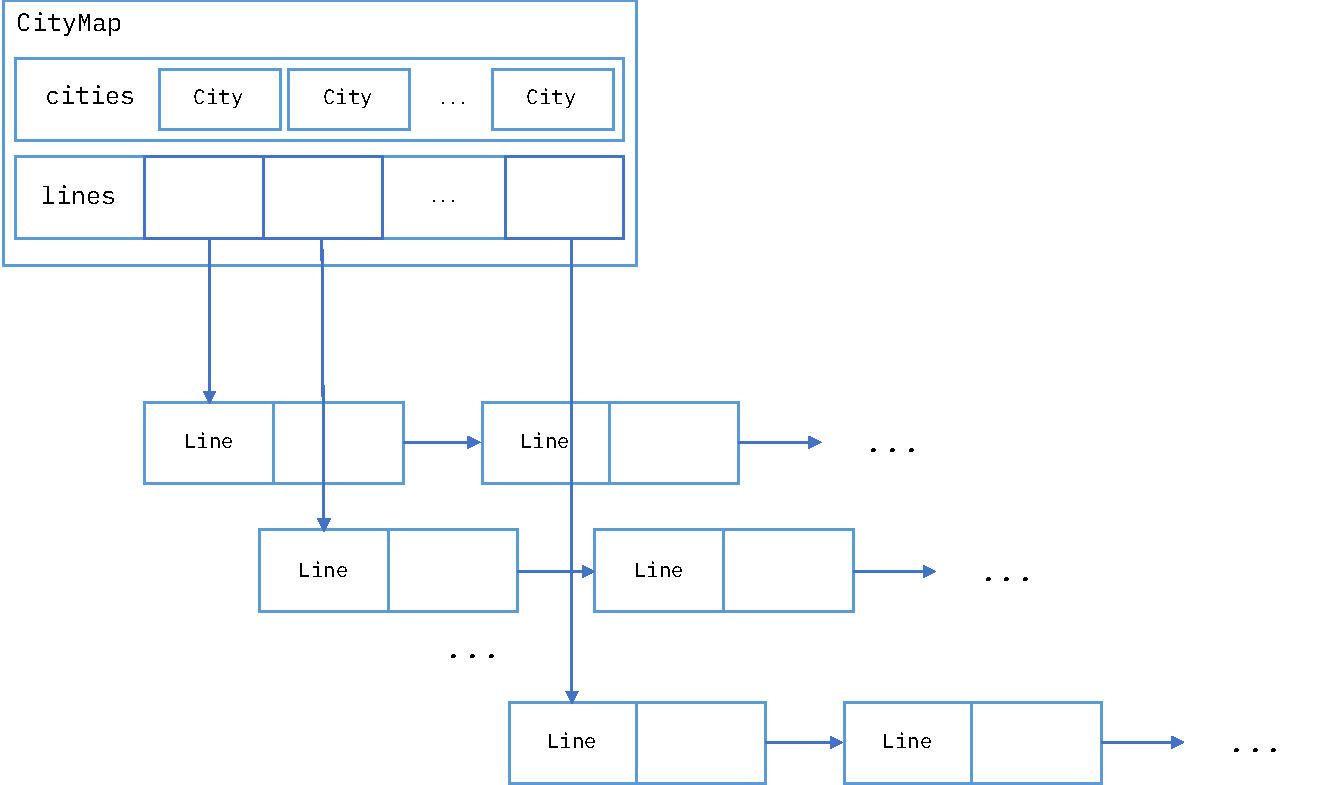
\includegraphics[width=0.7\textwidth]{figures/city_map_structure}
  \caption{城市线路图数据结构示意图}
  \label{fig:city-map-structure}
\end{figure}

实现中使用了C++的Template特性来使其能够适应不同的元素类型。

具体地,邻接表是一种利用链表存储图结构的数据结构,具有很好的空间复杂度。形式化地,
\begin{definition}[邻接表]
  对于一张图$\mathcal G = (\mathcal V, \mathcal E)$。利用一个映射$\varphi : \mathcal V \rightarrow \text{LinkedList<} \mathcal E \text{>}$来表示图的结构。具体地,$\varphi = c \mapsto \text{LinkedList} \{ l \in \mathcal E | c_s(l) = c \} $。也即为每一个节点映射一个存储边信息的链表,每一链表中包含对应节点出发的所有边。在实践中,映射往往由连续数组实现。
\end{definition}

对使用了邻接表存储的图而言,空间复杂度约为$\mathcal O(| \mathcal E |)$,对于一般的稀疏图而言,远远低于使用邻接矩阵存储的$\mathcal O(| \mathcal V |^2)$。

图 \ref{fig:city-map-structure} 中直观展示了城市线路图数据结构的主体结构。可以看到,数据结构中首先以数组存储了所有城市节点的信息。随后,以数组存储每一个城市的邻接表。每个城市的邻接表中保存了从该城市出发的所有线路信息。

\subsubsection{旅行方案}

旅行方案的本质是记录需要搭乘的线路。除此以外,还需要记录如出发地、目的地、总时长、风险值等辅助信息,方便接下来的处理。考虑到规划算法乃至于整套系统运行过程中,旅行方案有一个非常重要的特征:\textbf{在规划、生成旅行方案,乃至于接下来处理、展示方案的过程中,只涉及方案的生成、步骤的增添、路线的增长,不涉及对旅行方案中已有步骤的修改。}而另一个事实是,\textbf{在运行规划算法的过程中,会产生许多的临时、中间方案,而很多方案是从同一个中间方案延伸出来的,这些方案的路线中包含共享的部分。}

\paragraph{可持久化链表} 基于上面的特征和事实,我利用了\emph{可持久化链表 (persistent linked list)}来描述旅行方案。可持久化链表为可持久化数据结构中的一种,是\emph{无法原地修改 (immutable)}的数据结构。无法在原地修改的含义为,在修改时总是产生一个新的副本,而非在原来的链表上进行修改。这意味着无论在任何时候,先前产生的链表都不会因为后面产生的修改而被意外的改动。

可持久化链表在增加节点时非常简单。由于可持久化的性质保证了之前的链表不可能被修改,因而共享了元素的链表可以直接共用相同的部分。这带来了时间与空间上的优势。

\begin{figure}[t]
	\centering
	\subfloat[修改前]{
		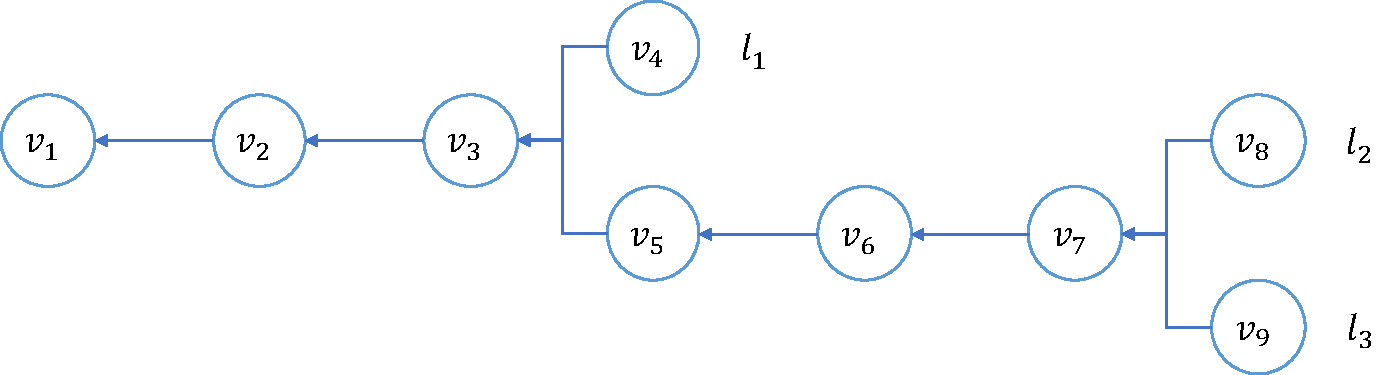
\includegraphics[width=0.5\textwidth]{figures/pll_example}
		\label{fig:pll-example-before}
	}
	\subfloat[修改后]{
		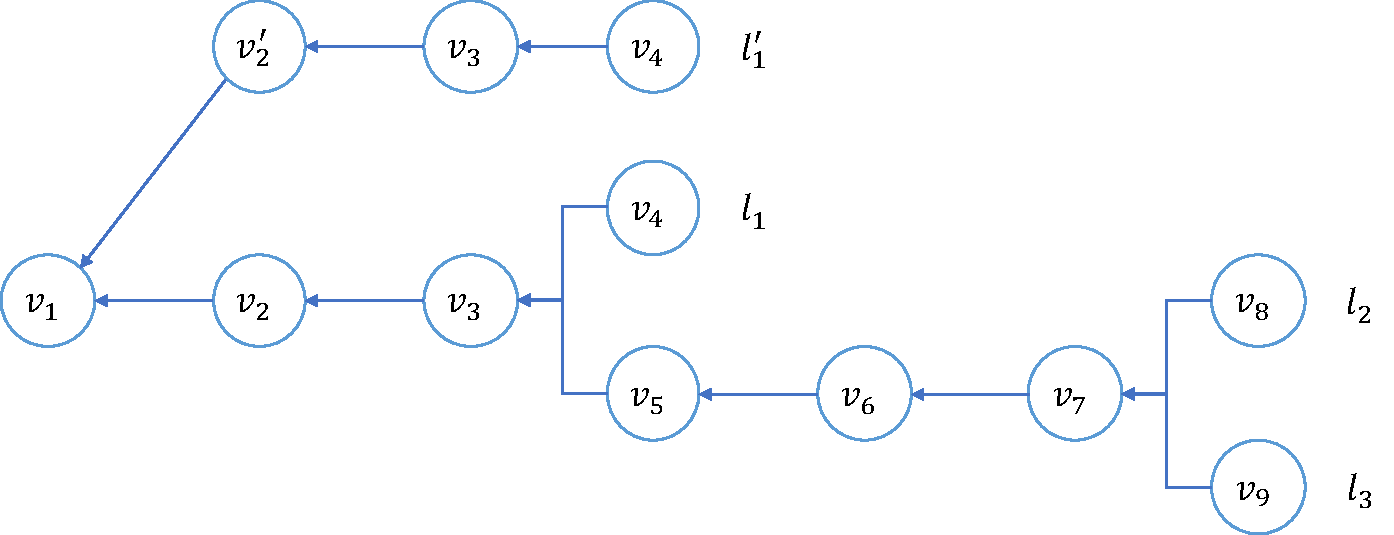
\includegraphics[width=0.5\linewidth]{figures/pll_example_mod}
		\label{fig:pll-example-mod}
	}
	\caption{可持久化链表的修改}
	\label{fig:pll-example}
\end{figure}

然而,在需要对链表的某一中间节点进行修改时将产生大量的复制。图 \ref{fig:pll-example-before} 中是采用了可持久化结构的三个链表。如果要将链表$l_1$从$v_4 \rightarrow v_3 \rightarrow v_2 \rightarrow v_1$修改为$v_4 \rightarrow v_3 \rightarrow v_2^\prime \rightarrow v_1$也即图 \ref{fig:pll-example-mod} 中的$l_1^\prime$,则需要将除了$v_1, v_2$之外的部分都进行复制。原因是在可持久化链表中,不能对之前的某个节点进行修改。

\paragraph{用可持久化链表描述旅行方案}

然而,在\textsc{TravelAgency}中,用可持久化链表来描述旅行方案可以规避上面提到的弱点:在规划的过程中,并不涉及对之前节点的修改,只涉及链表的延伸。因而在此应用场景中,可持久化链表能够实现高效的内存共享,快速的链表延伸,非常适合用于描述旅行方案。

具体地,旅行方案的数据结构可以如下表达。

\begin{lstlisting}[caption={旅行方案数据结构}]
struct Journey
{
  const int src; // 出发城市编号。
  const int dest; // 目的城市编号。
  const int dep_time; // 出发时间。
  const int arrive_time; // 到达时间。
  const int line; // 乘坐线路。
  const int length; // 总时长。
  const double risk; // 风险。
  const Journey *prev; // 上一段旅途方案。
}
\end{lstlisting}

\begin{algorithm}[t]
\caption{\textsc{Concat}($j$, $l$): $\mathcal J \times \mathcal E \rightarrow \mathcal J$}
\label{algo:concat-journey}
\KwIn{$j \in \mathcal J$:上一段的旅程方案;$l \in \mathcal E$:下一步搭乘的线路}
\KwOut{$j^\prime$:新的旅程方案}
\textsc{Assert}($j.dest = c_s(l)$)\;
$j^\prime.src \gets j.src$\;
$j^\prime.dest \gets c_d(l)$\;
$j^\prime.dep\_time \gets  j.dep\_time$\;
$j^\prime.arrive\_time \gets t_d(l) \oplus \tau(d)$\tcp*{$\oplus$ is mod-24 addition}
$j^\prime.line \gets l$\;
$j^\prime.length \gets j.length + \| t_d(l) - j.arrive\_time \| + \tau(l)$\;
$j^\prime.risk \gets j.risk + r_c(j.dest)\| t_d(l) - j.arrive\_time \| + r_l(l) r_c(j.dest) \tau(l)$\;
$j^\prime.prev \gets j$\;
\Return $j^\prime$\;
\end{algorithm}

而延伸旅行方案的算法如算法 \ref{algo:concat-journey} 中所示。其中$\mathcal J$为旅行方案的集合。注意到在数据结构定义中,所有的域都是不可修改的。算法中的赋值类似于初始化的过程,一旦完成赋值,离开算法,旅行方案中的域都无法修改。

\paragraph{可持久化链表的实现}

在实际的实现中,利用了C++中提供的 \lstinline{shared_ptr}。其最大的优势在于,能够方便、高效、不易出错地管理对同一片内存空间的引用。对算法运行过程中,产生的旅行方案的任一部分,只要当前的作用域内还包含对其的直接或间接引用,它就会被保留。当不再有对某一部分的任何引用时(如因发现更优解而将原先的解丢弃),将直接释放其内存。既不会产生内存泄漏,也不会对某一片内存产生多次或提前释放,产生不可预知的错误。

\subsection{算法核心中两种策略的规划算法}

\subsubsection{最小风险旅行规划算法}

\textsc{TravelAgency}系统中,最小风险规划算法的设计基于\emph{SPFA (shortest path faster algorithm)},也即带有队列优化的\emph{Bellman-ford}算法。是非常常用、高效的图上单源最短路算法。

然而,为了进行最小风险规划,系统并不直接在城市图上运行SPFA算法,而是在时间-城市图上。时间-城市图从城市图生成,其中的每一个节点都是包含了当前城市和当前时间的偶对。

\begin{wrapfigure}{r}{0.57\textwidth}
\begin{minipage}{0.57\textwidth}
\begin{algorithm}[H]
\caption{\textsc{ConstructTemporalEdges}($\mathcal G$)}
\label{algo:construct-temporal-edges}
\KwIn{$\mathcal G$: 输入城市图}
\KwOut{$\mathcal E^\prime$:时间-城市图的边集}
$\mathcal E^\prime \gets \emptyset$\;
\For{$e \in \mathcal E$}{
  $t_a \gets t_d(e) \oplus \tau(e)$\;
  $c_1 \gets c_s(e)$\;
  $c_2 \gets c_d(e)$\;
  \For{$t \in \mathds H$}{
    $\mathcal E^\prime \gets \mathcal E^\prime \cup \{ \langle (c_1, t), (c_2, t_a) \rangle \}$\;
  }
}
\Return $\mathcal E^\prime$\;
\end{algorithm}
\end{minipage}
\end{wrapfigure}

\begin{definition}[时间-城市图]
  对于一张城市图$\mathcal G = (\mathcal V, \mathcal E, r_c, r_l, t_d, t_a, \tau, v_s, v_d)$,其对应的时间-城市图为$\mathcal G^\prime = (\mathcal V^\prime, \mathcal E^\prime)$。其中$\mathcal V^\prime =  \mathcal V \times \mathds H$。其中$\mathds H \triangleq \{ 0, 1, \cdots, 23 \}$为一天中可能的时刻集合。集合$\mathcal E^\prime$的生成由算法 \ref{algo:construct-temporal-edges} 描述。注意,$t \oplus \tau \triangleq (t + \tau) \% 24$为模24加法。在模24加法下可以计算出线路的抵达时刻。
\end{definition}

\begin{figure}[t]
  \centering
  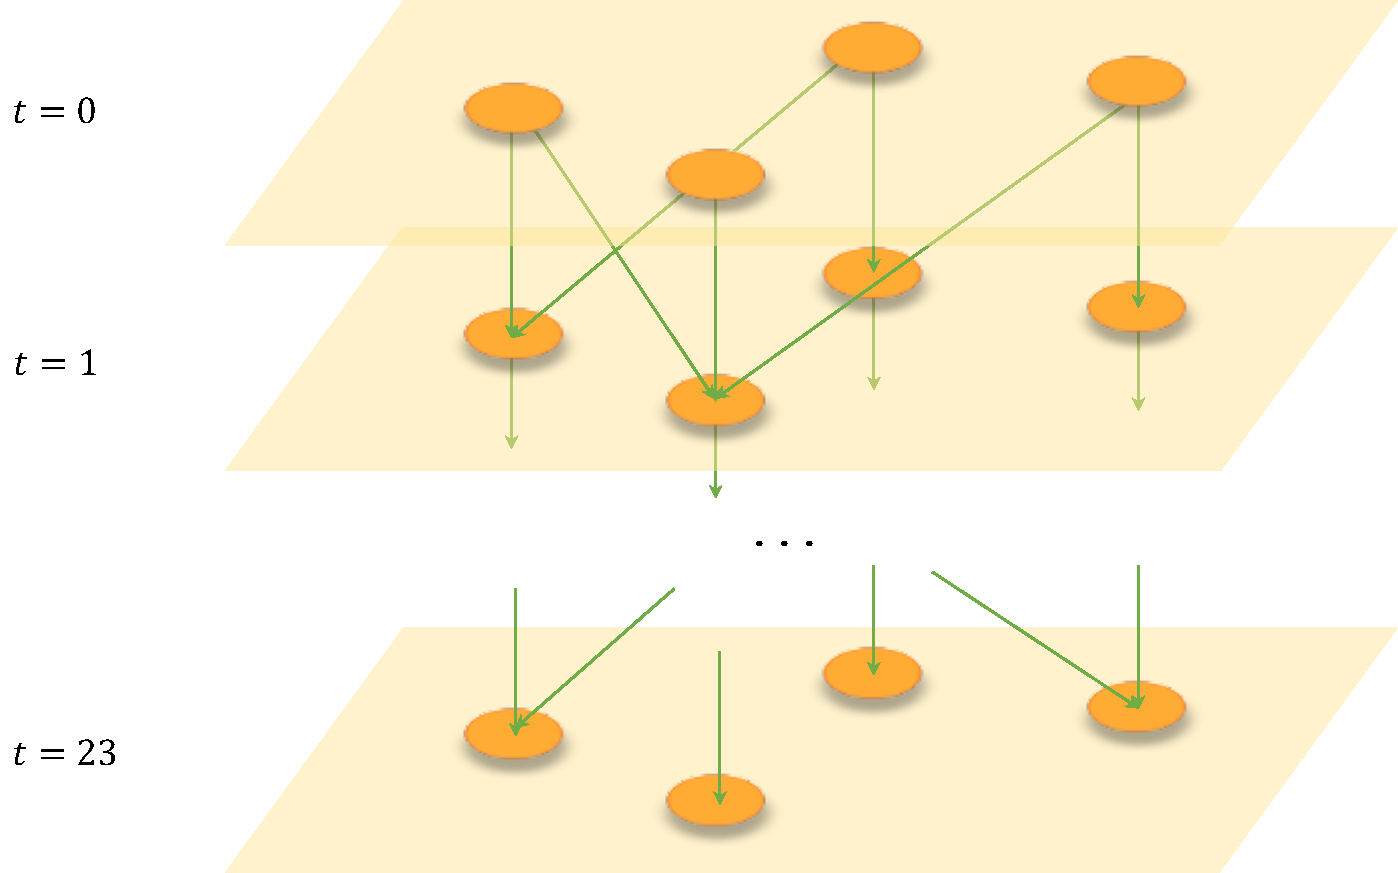
\includegraphics[width=0.7\textwidth]{figures/time_map}
  \caption{时间-城市图}
  \label{fig:time-map}
\end{figure}

图 \ref{fig:time-map} 中是一张时间-城市图的例子。其中的每一层都代表了一个时刻。图中的每个节点不仅包含城市信息,也有对应的时刻。图中的边不止是在城市之间转移,也在不同的时刻之间转移。使用时间-城市图,而非简单的城市图,能够更加准确、全面地描述出旅行中的状态信息。当某一旅客处于节点$(c, t)$时,则代表他当前处于城市$c$,当前时刻为$t$。在获知了当前时间$t$和当前地点$c$之后,旅客乘坐从当地出发的各条线路需要的等待时间、等待风险等,便可以明确地计算出来,乃至于从状态$(c, t)$到其他状态的最小风险路径,也可以通过算法方便地求解出来。

\begin{algorithm}[t]
\caption{\textsc{MinRiskSolver}($\mathcal G, c_1, c_2, t_0$)}
\label{algo:min-risk-solver}
\KwIn{$\mathcal G$:输入城市图;$c_1, c_2$:出发城市、目的城市;$t_0$:出发时间}
\KwOut{$j$:旅行方案}
$\bm J \in \mathcal J^{ |\mathcal V| \times |\mathcal H| }$\;
$\bm J[c_1, t_0] \gets $\textsc{Initial}($c_1, t_0$)\;
$q \gets $\textsc{Queue}$[ ]$\;
\textsc{Push}($q, \langle c_1, t_0 \rangle$)\;
\While{$q$ is not empty}{
  $\langle c, t \rangle \gets $\textsc{Pop}($q$)\;
  \For{$e \in \{ e_0 \in \mathcal E \mid c_s(e_0) = c \}$}{
    $j \gets $\textsc{Concat}$(\bm J[c, t], e)$\;
    $\langle c^\prime, t^\prime \rangle \gets \langle j.dest, j.arrive\_time \rangle$\;
    \If{$\langle c^\prime, t^\prime \rangle$ has not been reached $\vee \ j.risk < \bm J[c^\prime, t^\prime].risk$}{
      $\bm J [c^\prime, t^\prime] \gets j$\;
      \If{$\langle c^\prime, t^\prime \rangle \notin q$}{
        \textsc{Push}($q, \langle c^\prime, t^\prime \rangle$)\;
      }
    }
  }
  $j \gets $ empty\;
  \For{$t \in \mathds H$}{
    \If{$\bm J[c_2, t]$ is not empty}{
      \If{$j$ is empty $\vee$ $j.risk > \bm J[c_2, t].risk$}{
        $j \gets \bm J[c_2, t]$\;
      }
    }
  }
  
  \Return $j$\;
}
\end{algorithm}

求解最小风险策略旅行方案的算法如算法 \ref{algo:min-risk-solver} 中所示。算法并没有设计显示地构造时间-城市图的边集,因为这张图可以是一张\emph{隐含}图。在SPFA算法中要进行状态转移,更新状态最优解的时候,可以根据城市线路图中的边隐含地计算出时间-城市图中的边并进行处理。因而,时间-城市图中的边结构在算法运行的始末都不曾被显示地构造出来,这样将其视为隐含图的处理提高了算法的时间与空间效率。基于SPFA的算法 \ref{algo:min-risk-solver} 中使用了队列数据结构。其具有这些方法:\textsc{Queue}能够从一个列表构造出一个队列;\textsc{Push}($q, v$)将元素$v$放入队列$q$中;\textsc{Pop}($q$)从队列$q$中取出一个元素并返回。

算法 \ref{algo:min-risk-solver} 中使用的\textsc{Initial}方法,定义如算法 \ref{algo:initial} 中所示,作用是生成一个包含出发地点的初始化节点,供后续的算法处理。

\subsubsection{限时最小风险旅行规划算法}

\begin{wrapfigure}{r}{0.5\textwidth}
\begin{minipage}{0.5\textwidth}
\begin{algorithm}[H]
\caption{\textsc{Initial}($c_0$, $t_d$)}
\label{algo:initial}
\KwIn{$c_0$: 起始城市;$t_d$:出发时间}
\KwOut{$j$:供后续算法处理的起始旅行方案}
$j.src \gets c_0$\;
$j.dest \gets c_0$\;
$j.dep\_time \gets t_d$\;
$j.arrive\_time \gets t_d$\;
$j.line \gets $ null\;
$j.length \gets 0$\;
$j.risk \gets 0$\;
$j.prev \gets $ null\;
\Return $j$\;
\end{algorithm}
\end{minipage}
\end{wrapfigure}

限时最小风险策略的规划算法,同样能够基于SPFA实现。一个直觉的想法是在最小风险策略SPFA的状态更新过程中,直接丢弃超时的方案。这样可以保证能求出合法的解,然而却是错误的。下面给出一个反例。

\textbf{时间-城市图上带时间约束的SPFA算法的反例} \quad 考虑图 \ref{fig:bad-graph-example} 中的例子。若要求从$v_1$到$v_3$的限时最小风险路径,7点整出发,限制时间为30h,假设$v_1$到$v_2$有两种方案,一条时长为1h,风险为2;另一条时长为25h,风险为1。从$v_2$到$v_3$的最佳方案耗时6h,风险为2。通过肉眼观察可以发现,最佳路径时长为7h,风险为4。
\begin{figure}[t]
\centering
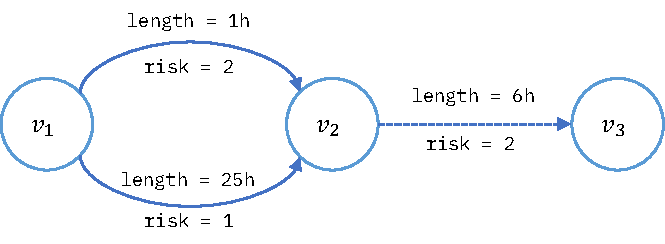
\includegraphics[width=0.7\textwidth]{figures/bad_graph_example}
\caption{例子}
\label{fig:bad-graph-example}
\end{figure}
然而在SPFA算法运行过程中,由于时长为1h的路径的风险大于另一条,时长为1h的路径会被丢弃,导致算法找不到可行解,错误地认为不可能在限制时间内到达目的地。

\textbf{时长-城市图} \quad 要解决上述问题的方法很简单,只需要将原本的时间-城市图,改为时长-城市图。也即图中的每一节点,从原先的包含当前时间与当前所在城市,改为当前从旅途开始已经过去的时间。对于某一城市图$\mathcal G$,限制时间为$\Gamma$,定义$\mathds D(\Gamma) \triangleq \{ 0, 1, 2, \cdots, \Gamma \}$,则时长-城市图的点集$\mathcal V^\prime = \mathcal V \times \mathds D(\Gamma)$,边集也可以像时间-城市图那样定义,并且无需显式构造。

限时最小风险的旅行规划算法与最小风险算法相类似。区别是节点定义的变化,以及在状态更新时需要考虑时长。具体定义如算法 \ref{algo:limited-time-min-risk-solver} 中所示。

\begin{algorithm}[t]
\caption{\textsc{LimitedTimeMinRiskSolver}($\mathcal G, c_1, c_2, t_0, \Gamma$)}
\label{algo:limited-time-min-risk-solver}
\KwIn{$\mathcal G$:输入城市图;$c_1, c_2$:出发城市、目的城市;$t_0$:出发时间;$\Gamma$:时间限制}
\KwOut{$j$:旅行方案}
$\bm J \in \mathcal J^{ |\mathcal V| \times |\Gamma + 1| }$\;
$\bm J[c_1, 0] \gets $\textsc{Initial}($c_1, t_0$)\;
$q \gets $\textsc{Queue}$[ ]$\;
\textsc{Push}($q, \langle c_1, 0 \rangle$)\;
\While{$q$ is not empty}{
  $\langle c, t \rangle \gets $\textsc{Pop}($q$)\;
  \For{$e \in \{ e_0 \in \mathcal E \mid c_s(e_0) = c \}$}{
    $j \gets $\textsc{Concat}$(\bm J[c, t], e)$\;
    $\langle c^\prime, t^\prime \rangle \gets \langle j.dest, j.length \rangle$\;
    \If{$j.length \leq \Gamma$ $\wedge$ $(\langle c^\prime, t^\prime \rangle$ has not been reached $\vee \ j.risk < \bm J[c^\prime, t^\prime].risk)$}{
      $\bm J [c^\prime, t^\prime] \gets j$\;
      \If{$\langle c^\prime, t^\prime \rangle \notin q$}{
        \textsc{Push}($q, \langle c^\prime, t^\prime \rangle$)\;
      }
    }
  }
  $j \gets $ empty\;
  \For{$t \in \mathds D(\Gamma)$}{
    \If{$\bm J[c_2, t]$ is not empty}{
      \If{$j$ is empty $\vee$ $j.risk > \bm J[c_2, t].risk$}{
        $j \gets \bm J[c_2, t]$\;
      }
    }
  }
  
  \Return $j$\;
}
\end{algorithm}

\subsubsection{算法性能分析}

最小风险与限时最小风险规划算法都基于SPFA。查阅资料可知SPFA在实验中的平均时间复杂度约为$\mathcal O(|\mathcal E^\prime|)$,最坏时间复杂度为$\mathcal O(|\mathcal V^\prime| |\mathcal E^\prime|)$其中$\mathcal V^\prime, \mathcal E^\prime$分别为隐含图的点集与边集。

因而,对于最小风险策略规划算法而言,可以认为算法的时间复杂度约为$\mathcal O(|\mathds H| |\mathcal E|) = \mathcal O(|\mathcal E|)$。对于限时最小风险规划算法而言,时间复杂度约为$\mathcal O(| \Gamma + 1 | | \mathcal E |)$。他们关于线路数量都是线性的。

\subsection{服务器的设计}

本小节将介绍服务器的功能与设计实现。首先介绍功能。
\begin{enumerate}[(a)]
  \item 存储规划好的旅程信息。服务器将保存算法核心规划好的旅程信息,存入旅程列表。并且在前端界面要求的时候发送给前端,由前端展现给用户。
  \item 与前端界面通信。服务器需要响应前端请求,返回相应数据。
  \item 调用算法核心中的算法。服务器通过加载动态库,来调用算法核心实现的算法,进行旅行方案的规划。
\end{enumerate}

\begin{figure}[t]
  \centering
  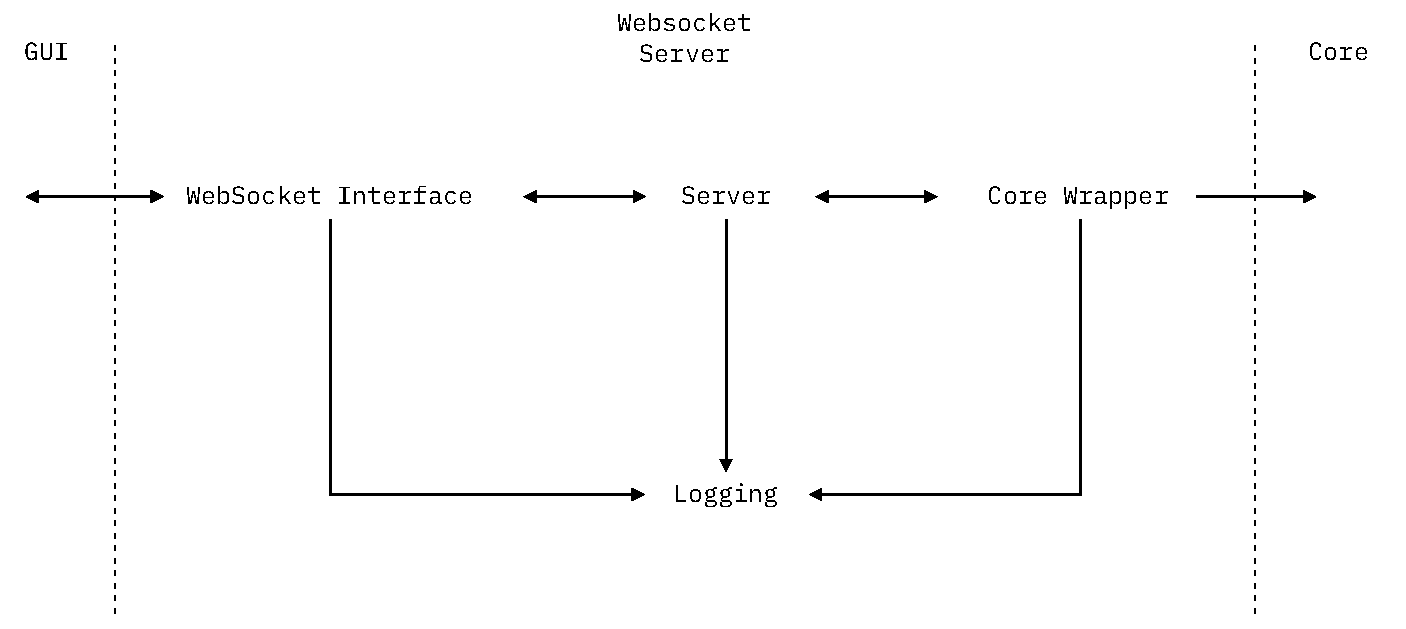
\includegraphics[width=0.7\textwidth]{figures/server_arch}
  \caption{服务器模块结构图}
  \label{fig:server-arch}
\end{figure}

{\setstretch{1.5}
服务器的模块结构图如图 \ref{fig:server-arch} 中所示。服务器主要有如下模块。
\begin{enumerate}[(a)]
  \item \textbf{WebSocket接口 (WebSocket Interface)}。该模块负责与前端进行通信。使用Python的 \lstinline{websockets} 与 \lstinline{asyncio} 库实现。考虑到接口的负载并不大,一般而言只有一个前端与之通信,因而 \lstinline{asyncio} 提供的并发实现完全足够。
  \item \textbf{服务器 (Server)}。服务器模块包含对前端请求的处理逻辑,以及包含了对服务器状态(动态库接口句柄,旅行方案列表等)的定义与管理。
  \item \textbf{日志记录 (Logging)}。由Python的 \lstinline{logging} 库实现。能够对日志信息进行分级记录与显示。
  \item \textbf{核心库封装 (Core Wrapper)}。核心库封装模块通过 \lstinline{ctypes} 调用C++编写的动态库,并且将其中的函数封装为Python函数,将C++中定义的数据结构映射到Python中,定义相应的类。
\end{enumerate}}

\subsection{前端用户界面的设计}

前端界面主要要实现如下功能:
\begin{enumerate}
  \item 接受用户输入,交互式地添加、查看旅行。
  \item 实时显示城市信息、旅行状态,显示旅行线路、展示旅客状态等。
  \item 与服务器进行通信,添加旅行方案,要求规划旅行方案,要求获取城市、道路信息等。
  \item 管理当前时间状态,暂停、继续当前时间的进行,根据当前时间计算出各个旅程所处的状态等。
\end{enumerate}

\begin{figure}[t]
  \centering
  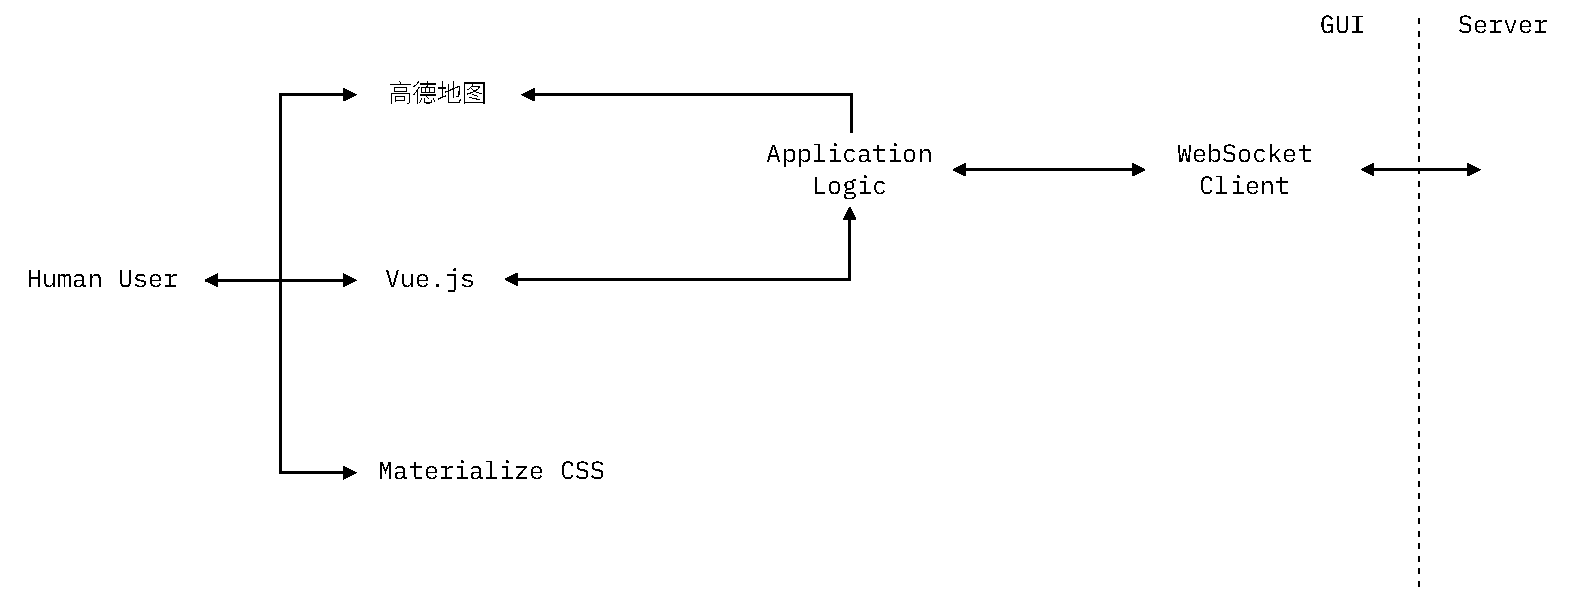
\includegraphics[width=0.7\textwidth]{figures/gui_arch}
  \caption{前端界面模块结构图}
  \label{fig:gui-arch}
\end{figure}

前端界面的模块结构如图 \ref{fig:gui-arch} 中所示。其功能分别如下:
\begin{enumerate}
  \item \textbf{高德地图、Vue.js、Materialize CSS}。这三个模块都负责前端界面的显示与交互。高德地图负责地图的显示、城市信息的绘制、旅程信息的绘制等等。Vue.js是非常常用的前端框架,负责右侧信息面板的交互事件管理与数据的渲染。并且也监听程序状态的变化,若有必要将根据变更的状态在高德地图中重新渲染。Materialize CSS也是常用的前端界面框架,能够提供Material Design风格的前端组件。
  \item \textbf{程序逻辑 (Application Logic)}。该模块实现了程序的主体逻辑。如如何响应用户事件、调用WebSocket客户端进行通信、如何响应WebSocket信息等等。并实现了地图的绘制逻辑。
  \item \textbf{WebSocket客户端 (WebSocket Client)}。该模块负责建立WebSocket连接,与服务器通信。
\end{enumerate}























\section{样例运行结果与测试}
\label{sec:experiments}

\subsection{样例城市线路信息}

\textsc{TravelAgency}系统使用的样例城市线路信息包含14个城市,540条线路。14个城市分别为:北京、青岛、银川、南京、上海、杭州、西安、武汉、长沙、广州、南宁、重庆、昆明、拉萨。包括了全国各大主要城市、大多数省会城市等等。

\begin{table}[h]
\centering
\begin{tabular}{cccc}
\toprule
航班班次 & 列车班次 & 客车班次 & 总计 \\
\midrule
10 & 30 & 500 & 540 \\
\bottomrule
\end{tabular}
\caption{线路班次数量}
\label{tab:line-info}
\end{table}

表 \ref{tab:line-info} 中给出了线路的基本信息。除了航班是根据城市重要程度人为指定以外,火车、客车的班次,是在事先划定了连通的城市之后,根据数量随机生成的。线路的时间是根据两地之间的距离以及线路类型生成的,而线路的出发时间都是在集合$\mathds H$中随机选择的。

\subsection{一个例子:从拉萨到杭州的旅行方案}

\begin{figure}[t]
	\centering
	\subfloat[最小风险策略方案]{
		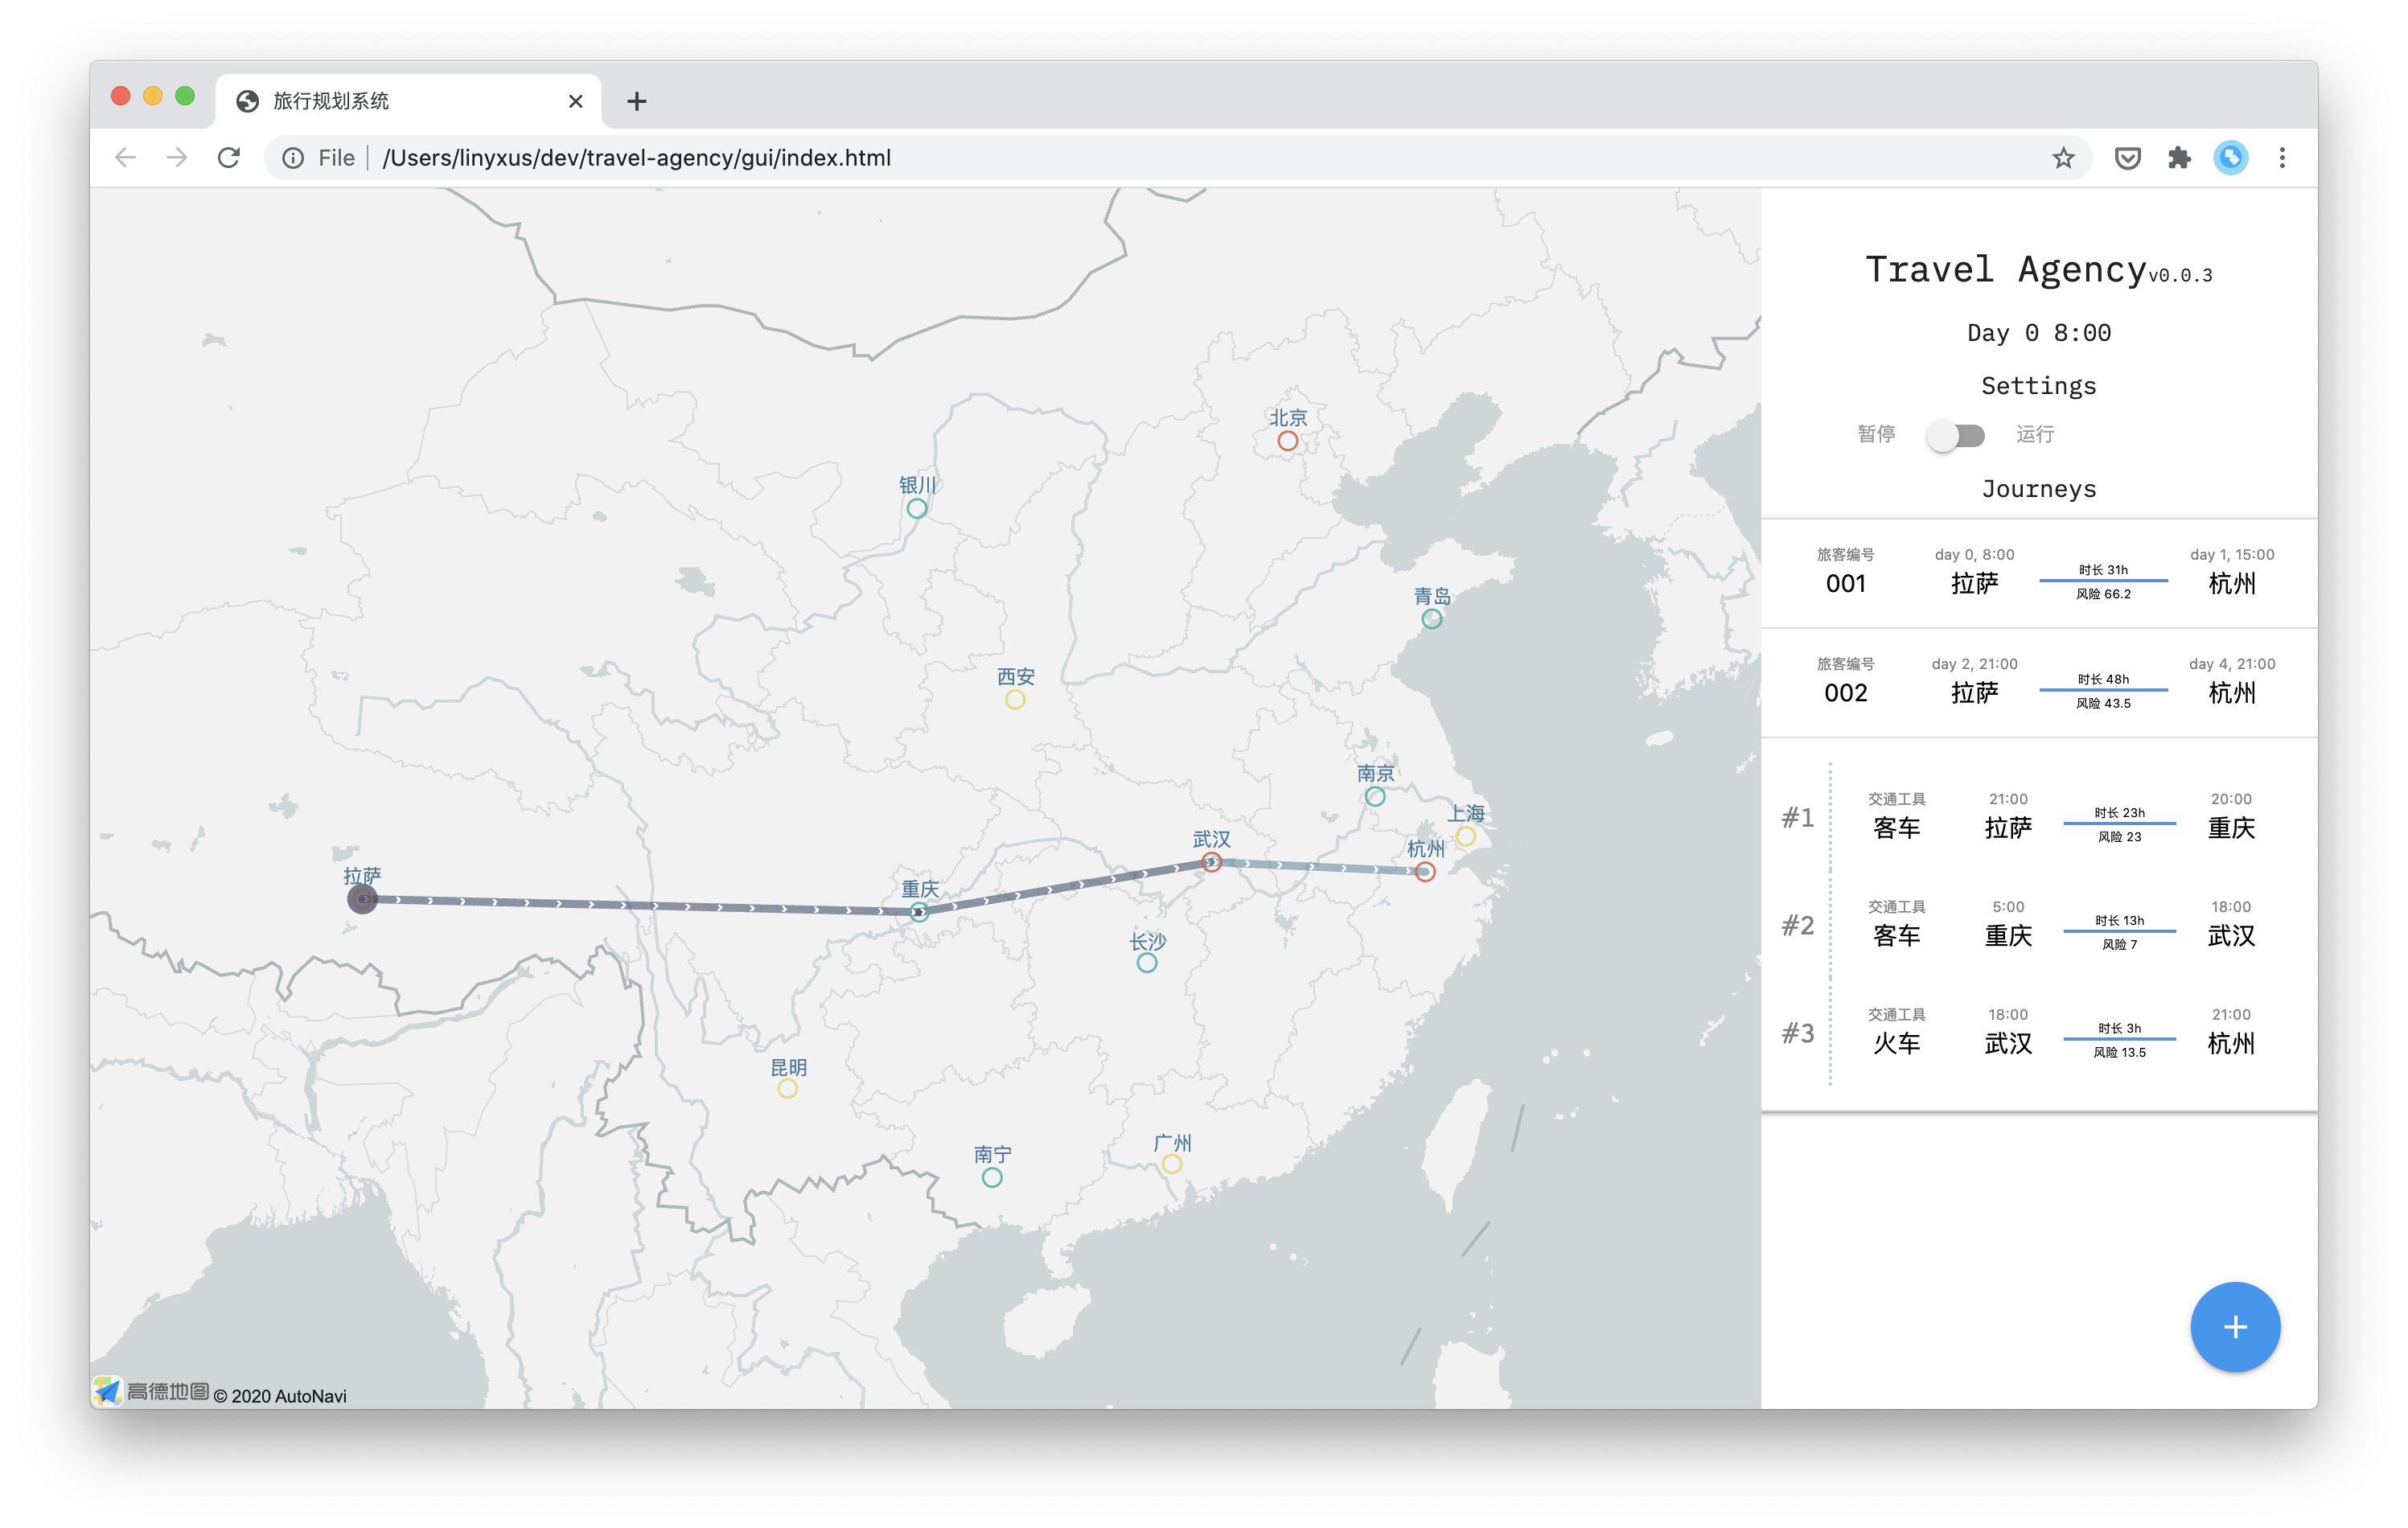
\includegraphics[width=0.5\textwidth]{figures/example_journey_mr}
		\label{fig:example-journey-mr}
	}
	\subfloat[限时最小风险策略方案]{
		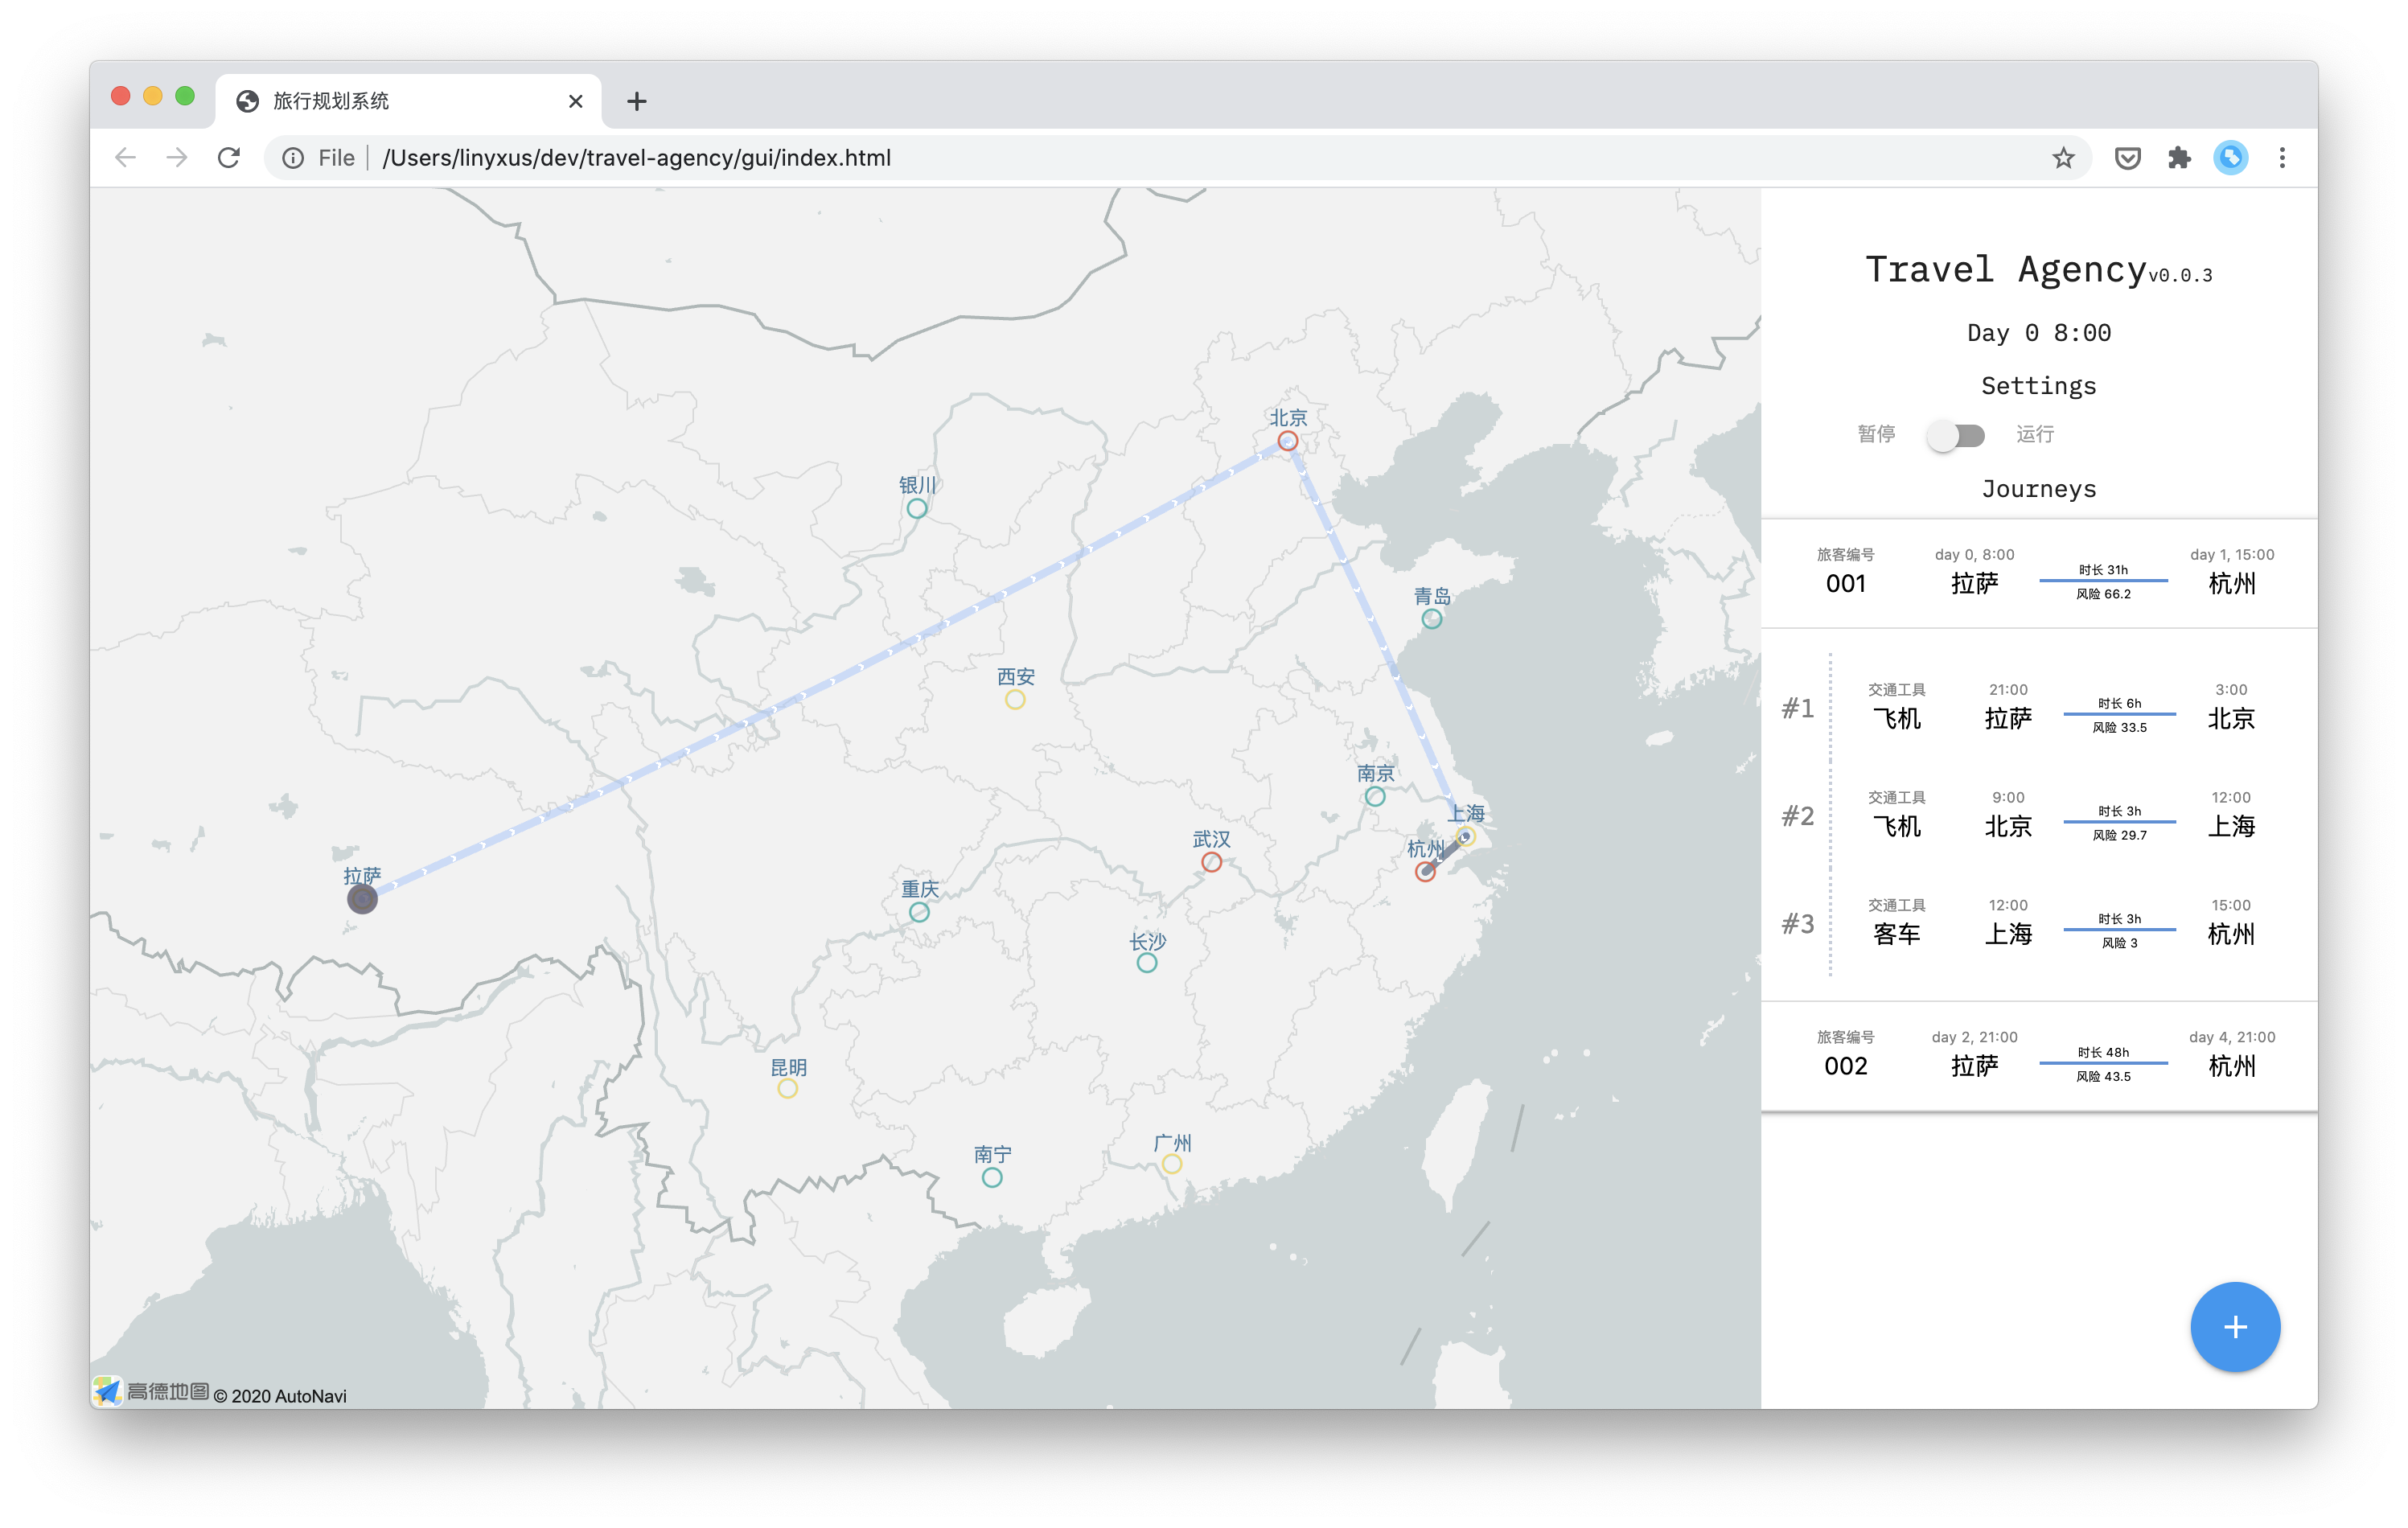
\includegraphics[width=0.5\linewidth]{figures/example_journey_ltmr}
		\label{fig:example-journey-ltmr}
	}
	\caption{从拉萨到杭州的旅行方案}
	\label{fig:example-journey}
\end{figure}

如图 \ref{fig:example-journey} 中所示,我给出了一个利用\textsc{TravelAgency}系统进行旅行规划的例子。例子中规划了从拉萨到杭州的旅行方案,图 \ref{fig:example-journey-mr} 中给出了最小风险策略的方案,图 \ref{fig:example-journey-ltmr} 中给出了限时40小时的最小风险方案。从图中可以看出,最小风险方案虽然风险最小,但是绕了远路,导致超出时间限制(需要48小时),而限时最小风险方案走了较为近的路程,且更多搭乘飞机,导致风险更大一些。

\subsection{单元测试}

在开发过程中,为C++编写的主要模块,借助GoogleTest测试框架编写了单元测试。主要有如下测试集:
\begin{enumerate}[(a)]
  \item \textbf{\lstinline{CityMap}模块。} 主要测试了城市线路信息能否正确读取、处理。
  \item \textbf{\lstinline{Journey}模块。} 主要测试了Journey类的关键方法,是否正确构造,是否能正确转化为线路列表,是否正确求出风险值等等。
  \item \textbf{\lstinline{LinkedList}模块。} 主要测试了链表类的关键方法。能否正确添加元素、求长度等等。
  \item \textbf{\lstinline{Solver}模块。} 测试了两种旅行规划模块能否给出正确的结果。
\end{enumerate}
共有5个测试集,22个测试点。测试了系统的核心功能,保证代码质量。为了运行测试,需要首先编译工程,随后在工程的根目录内运行 \texttt{./build/default/test\_main}。工程可以通过所有测试点。











\section{总结}
\label{sec:conclusion}

本报告中,我阐述了疫情环境下低风险旅行规划模拟系统\textsc{TravelAgency}的背景、目的、主要功能、具体设计、开发过程等。\textsc{TravelAgency}是一个实用高效、简洁美观的旅行规划系统。能够基于两种不同的旅行策略(最小风险、限时最小风险)进行旅行方案的规划,并且能实时地显示出各个旅客的旅程状态。这一系统由三大模块组成:前端界面、服务器、算法核心。采用了丰富的技术栈,进行了高效的开发,在算法核心中使用了图、链表、可持久化链表、队列等数据结构。并应用SPFA算法,在隐含的时间-城市图、时长-城市图上求解最优路径。

\textsc{TravelAgency}系统具有如下优点:
\begin{enumerate}[(a)]
  \item \textbf{功能齐全。} 系统实现了所有要求的功能,以及两个选做功能。能够读取、管理城市线路信息,进行两种策略的路径规划;能够实时显示各个旅客的旅行状态,且在规划的过程中,能够考虑到旅行途中带来的风险。
  \item \textbf{界面美观,简洁明了。} 系统利用前端技术实现了用户图形界面。调用了高德地图API,采用了Material Design风格的界面,美观大方,简洁明了,且能对需要的信息进行高效、清晰的展示。
  \item \textbf{采用了高效的数据结构与算法。} 系统采用了高效的数据结构与算法。利用邻接链表来表示城市线路图中的边;利用可持久化链表来表示旅程。并且使用了SPFA来进行旅行方案的规划。其平均时间复杂度可达到$\mathcal O(|\mathcal E^\prime|)$,最坏时间复杂度为$\mathcal O(|\mathcal V^\prime| |\mathcal E^\prime|)$。
  \item \textbf{模块划分明确,开发效率高。} 系统被划分为三个主要模块,使用不同的技术进行开发。用户界面由前端技术完成,效率高,界面美观;服务器由Python开发,Python具有成熟的WebSocket工具库与并发库,开发效率高;算法核心由C++进行开发,能够实现很高的时间、空间效率,且为编译型语言,运行效率高,保证核心算法的运行速度。因而,各大模块各司其职,且采取了合适的技术进行开发,兼顾了开发效率与系统质量。
\end{enumerate}

而另一方面,\textsc{TravelAgency}系统还有一些需要改进的不足之处:(1) 在功能方面,可以添加更多、更完善的功能,例如:添加用户的注册机制,让每一用户可以同时规划多个旅程,并只显示自己规划的旅程;在旅程进行过程中,增加修改目的地的功能,提高系统灵活性;考虑用户更加细致的需求,如不愿意乘坐飞机,以及追求时间最短等。(2) 在前端界面方面,可以考虑使用WebAssembly这样的新技术,来获得更高的效率。(3) 在服务器与后端接口方面,现在使用的是 \lstinline{ctypes} 对动态库进行调用,需要动态地设置需要调用的函数的参数、返回值信息,容易出错,难以维护,可以替换成 \lstinline{cffi} 在编译期进行库配置,具有更高的开发效率。

综上所述,\textsc{TravelAgency}是一个高效美观、设计良好的低风险旅行模拟规划系统。系统具有诸多优点,也有一些需要改进之处。设计、实现这一课程设计项目的过程让我获益良多,在之后的软件开发过程中,我将吸收其中的经验,更进一步。


\newpage

\begin{appendices}
\section{工程的编译与运行}
\label{sec:compile-and-run}

\subsection{环境要求}

以下是编译、运行所需要的工具要求:
\begin{itemize}
  \item Chrome 83+
  \item Python 3.7+
  \item CMake 3.17
  \item Ninja 1.10
\end{itemize}

Python依赖的第三方包如下:
\begin{enumerate}
  \item websockets 8.1
\end{enumerate}

项目的开发、测试环境为 macOS Catalina 10.15.5。\textbf{注意:在\texttt{./py/\_travel\_agency.py}文件中,硬编码了动态链接库的位置。在macOS下动态链接库的后缀名为\texttt{.dylib},如果在Windows下或者Linux下运行代码,要在编译动态库后将动态库文件名相应修改。}

\subsection{编译方法}

本项目中,C++算法核心部分使用CMake + Ninja工具链进行编译。前端界面与Python服务器均无需编译。C++动态库的编译过程如下。

首先,调用CMake生成编译文件。在项目根目录执行下列指令。
\begin{verbatim}
mkdir -p build/default
cd build/default
cmake -GNinja -DBUILD_SHARED_LIBS=ON ../..
\end{verbatim}

随后,调用Ninja进行编译。同样在项目根目录执行下列指令。
\begin{verbatim}
cd build/default
ninja
\end{verbatim}

Ninja将打印出编译的过程与结果。若编译顺利,\texttt{./build/default/} 文件夹内将生成动态库文件。

\textbf{注意:如果在Windows下编译,若发现编译产生的DLL文件出现了乱码现象,则需要在 \texttt{./src/travel\_agency.hh}文件中的函数定义中添加 \lstinline{\_\_declspec(dllexport)}宏。在类Unix环境下,只需要将函数定义包裹在 \lstinline{extern "C"} 中,编译器就不会对导出的函数名进行修饰,而在Windows下,添加上述宏是必要的。由于本项目在 macOS 下开发,因而没有添加这些宏。如果着手自己编译,需要注意这一点。}

\subsection{运行方法(预编译的Windows可执行文件)}

提交的文件中已经包含了预编译的Windows可执行文件。只需要双击运行,\textbf{并且根据给出的提示在浏览器中打开相应网页}即可以运行系统。

\subsection{运行方法(自行编译)}

在运行之前,请保证:
\begin{enumerate}
  \item 动态链接库已经正确编译,产生在\texttt{./build/default/}文件夹内。在Windows下,为\texttt{.dll}后缀的文件,在Linux下,为\texttt{.so},在macOS下,为\texttt{.dylib};
  \item 如果在Windows下或Linux下运行程序,需要根据编译生成的动态库路径,修改\texttt{./py/\_travel\_agency.py}文件中动态库的位置。
  \item 如果在Windows下运行程序,需要确保Python版本为3.7。若产生DLL加载错误,则很有可能是依赖的DLL没有放在Python的DLL加载路径中,如 \lstinline{libstdc++}等等。需要找寻到对应的DLL并放入加载目录。
\end{enumerate}

首先,运行Python服务器。
\begin{verbatim}
cd py
python main.py
\end{verbatim}

然后,在浏览器(推荐使用新版本的Chrome)中打开\texttt{./gui/index.html}文件。这可以通过打开链接:\texttt{file:///\$PROJECT\_PATH/gui/index.html}来实现。其中\texttt{\$PROJECT\_PATH}为项目文件夹所在路径。网页界面将自动连接服务器。系统开始运行。

\section{系统使用说明}
\label{sec:manual}

系统界面分为两个部分:地图与信息面板。地图上能够显示城市信息、旅程详细信息与状态等。信息面板则呈现各类信息,包括事件、旅行列表,也有添加按钮。接下来分点详细阐释系统功能与使用方法。

\textbf{查看城市信息。} \quad 在界面的地图部分上,用圆圈标出了系统支持的旅行城市。圆圈上方为城市名称。圆圈的颜色代表了城市的风险等级:\textit{{\color{high-risk}红色}}代表高风险地区;\textit{{\color{mid-risk}黄色}}代表中风险地区;\textit{{\color{low-risk}绿色}}代表低风险地区。

\textbf{查看时间信息、控制时间运行。} \quad 信息面板的上方给出了系统的当前时间。系统时间从第 0 天 0 时开始,以固定的间隔,以1小时为单位向前推进。下面的按钮能够暂停、重启系统时间的运行。

\definecolor{air}{HTML}{a0c4ff}
\definecolor{subway}{HTML}{457b9d}
\definecolor{highway}{HTML}{1d3557}

\textbf{旅行列表、查看旅行详情。} \quad 信息面板时间的下方,为旅行列表。旅行列表中的每一项都是正在进行中的旅程。列表中每一项都给出了旅程的简要信息,包括:旅客编号、出发时间、出发地点、到达时间、目的地点、旅行时长、旅行风险。点击列表中的某一项,将显示该旅程的详细信息,包括每一步搭乘的线路信息,线路时长,在线路中产生的风险等。同时,地图中将绘制出该条线路的详细路径。并且以灰色圆形指示旅客当前所处位置。绘制的路径中,\textit{\color{air}天蓝色}代表飞机,\textit{\color{subway}青色}代表火车,\textit{\color{highway}靛色}代表公路。将鼠标移到旅客标识上,将显示旅客状态。

\textbf{添加旅程。} \quad 点击右下角按钮,将打开添加旅程窗口,窗口打开后,将自动暂停系统时间。在窗口中需要输入旅程信息、选择旅行策略。当所有信息都被输入且合法时,将显示旅行预览,更新信息,旅行预览也会更新。当信息有问题(出发地、目的地相同,或找不到可行的方案)时,旅行预览不会显示。点击确认按钮,若信息无问题,系统将旅行添加到列表内;若信息有问题,将产生提示。点击取消按钮,将返回到主界面,输入的信息将被丢弃。

\textbf{查看系统日志。} \quad 在Python服务器终端内,可以看到系统日志。系统日志将打印出客户端的连接、断开信息;客户端的请求、服务器的响应信息;运行规划算法的信息与耗时;其他提示信息等。

\section{性能测试}
\label{sec:perf-test}

\begin{table}[t]
  \centering
  \resizebox{\textwidth}{!}{%
  \begin{tabular}{c|cccccc}
    \toprule
    项目 & 平均用时 (ms) & 最大用时 (ms) & 最小用时 (ms) & 平均空间 (MiB) & 最大空间 (MiB) & 最小空间 (MiB) \\
    \midrule
最小风险 & 18.10 & 29.84 & 10.44 & 70.39 & 71.53 & 64.89 \\
限时最小风险 & 33.42 & 58.50 & 8.58 & 115.06 & 129.33 & 71.38 \\
全部 & 25.76 & 58.50 & 8.58 & 92.73 & 129.33 & 64.89 \\
    \bottomrule
  \end{tabular}%
  }
  \caption{在随机生成的$10^4$座城市,$10^5$条线路的地图上的性能测试表现}
  \label{tab:perf-test}
\end{table}

为了进一步验证系统效率,我随机生成了大规模的城市图,在上面运行系统的规划算法,测量不同策略的规划时间与内存消耗。具体地,将城市数设为$10^4$,并随机生成$10^5$条线路,每种策略运行100次,性能测试的结果在表 \ref{tab:perf-test} 中给出。从中可以看出,在这一大规模的图上进行规划,算法仍然能够以非常快地速度给出结果,证明了系统中算法的高效性。




























\end{appendices}

\end{document}

















